\documentclass[a4paper,10pt]{article}
\usepackage[utf8]{inputenc}
\usepackage{amsmath}
\usepackage{fullpage}
\usepackage{hyperref}
\usepackage{graphicx}
\usepackage{listings}
\usepackage{color}

\definecolor{mygreen}{rgb}{0,0.6,0}
\definecolor{mygray}{rgb}{0.5,0.5,0.5}
\definecolor{mymauve}{rgb}{0.58,0,0.82}

\lstset{ 
  backgroundcolor=\color{white},   % choose the background color; you must add \usepackage{color} or \usepackage{xcolor}; should come as last argument
  basicstyle=\footnotesize,        % the size of the fonts that are used for the code
  breakatwhitespace=false,         % sets if automatic breaks should only happen at whitespace
  breaklines=true,                 % sets automatic line breaking
  captionpos=b,                    % sets the caption-position to bottom
  commentstyle=\color{mygreen},    % comment style
  deletekeywords={...},            % if you want to delete keywords from the given language
  escapeinside={\%*}{*)},          % if you want to add LaTeX within your code
  extendedchars=true,              % lets you use non-ASCII characters; for 8-bits encodings only, does not work with UTF-8
  firstnumber=1,                   % start line enumeration with line 1000
  frame=single,	                   % adds a frame around the code
  keepspaces=true,                 % keeps spaces in text, useful for keeping indentation of code (possibly needs columns=flexible)
  keywordstyle=\color{blue},       % keyword style
  language=Python,                 % the language of the code
  morekeywords={*,...},            % if you want to add more keywords to the set
  numbers=left,                    % where to put the line-numbers; possible values are (none, left, right)
  numbersep=5pt,                   % how far the line-numbers are from the code
  numberstyle=\tiny\color{mygray}, % the style that is used for the line-numbers
  rulecolor=\color{black},         % if not set, the frame-color may be changed on line-breaks within not-black text (e.g. comments (green here))
  showspaces=false,                % show spaces everywhere adding particular underscores; it overrides 'showstringspaces'
  showstringspaces=false,          % underline spaces within strings only
  showtabs=false,                  % show tabs within strings adding particular underscores
  stepnumber=1,                    % the step between two line-numbers. If it's 1, each line will be numbered
  stringstyle=\color{mymauve},     % string literal style
  tabsize=4,	                   % sets default tabsize to 2 spaces
  title=\lstname                   % show the filename of files included with \lstinputlisting; also try caption instead of title
}


\renewenvironment{abstract}
 { \vspace*{0.3cm} \textbf{\abstractname} \vspace{0.1cm} \\ \ignorespaces}
 {\par\medskip \vspace{0.1cm}}

\setlength{\parindent}{0em}

\setlength{\textheight}{25.7cm}
\setlength{\textwidth}{18cm}
\setlength{\unitlength}{1mm}
\setlength{\topskip}{2truecm}

\topmargin 260mm \advance \topmargin -\textheight
\divide \topmargin by 2 \advance \topmargin -1in
\headheight 0pt \headsep 0pt \leftmargin 210mm \advance
\leftmargin -\textwidth
\divide \leftmargin by 2 \advance \leftmargin -1in
\oddsidemargin \leftmargin \evensidemargin \leftmargin
\parindent=0pt
\frenchspacing


%opening
\title{\vspace{-1cm}\textbf{Numerical Recipes for Astrophysics \\ Solutions hand-in Assignment-2}}
\author{Luther Algra - s1633376}

\begin{document}

\maketitle
% two segments of code. The first segment of code contains the full code of the program that executes the sub-questions. The second segment contains the shared modules (if any) used by the sub-question.
\hrule
\begin{abstract}
The current document contains the solutions for the second hand-in assignment of Numerical Recipes. The main questions, 1, 2, 3 ..., 7, are in this document all given their own section. Each section contains a subsection for its related sub-questions (1.a, 1.b, 1.c, ..., 1.e) and ends with a final subsection that contains two segments of code. The first segment contains the code of the main question. The second segment contains the code of shared modules used by the sub-questions. A sub-question itself always starts with a short summary of the question that needs to be answered. The summary is followed by an explanation of how the problem is solved and the code that provides the solution. If necessary some of the results are discussed here. The output of the code is always presented after the code and plots are discussed in their caption.


\end{abstract}
\hrule
\vspace{0.5cm}


\section*{\textbf{1 - Normally distributed pseudo-random numbers} \hrule} 



\subsection*{\textbf{Question 1.a}}
\begin{quote}

\textbf{Problem}
\begin{quote}Write a random number generator that returns a random floating-point number between 0 and 1. At minimum, use some combination of an MWC and a 64-bit XOR-shift. Plot a sequential of random numbers against each other in a scatter plot ($x_{i+1}$ vs $x_{i}$) for the first 1000 numbers generated. Also plot the value of the random numbers for the first 1000 numbers vs the index of the random number, this mean the x-axis has a value from 0 through 999 and the y-axis 0 through 1). Finally, have your code generate 1,000,000 random numbers and plot the result of binning these in 20 bins 0.05 wide. 
\end{quote}

\textbf{Solution} 


\begin{quote}
The state of the random number generator is updated by first performing a 64-bit XOR-shift on the current state and then giving a modified version of the obtained output to the MWC algorithm. The modification of the XOR-shifts output consists of putting the last 32 bits to zero. This is done by performing the 'AND' operation with the maximum value of an unsigned int 32. This modification was performed as the  MWC algorithm expects as input a 64-bit unsigned integer with a value between  $0 < x < 2^{32}$.

The output of the MWC algorithm for this modified value is set as new state of the random number generator. The first 32 bits of the new state are used to provide a random value, as the output of the MWC algorithm only contains 32 significant bits. This random value is obtained by performing the 'AND' operation between the seed and the maximum value of an unsigned int 32. The resulting value is then divided by the maximum value of an uint32 to obtain a value between 0 and 1.

The code for the random number generator can be found at the end of this section, as it is treated as a shared module. The code for generating the plots and the created plots can be found below. 
\end{quote}
\newpage

\textbf{Code - Plots}


% consists of the code that initializes the random number generator and calls the function.

\begin{quote}
The code for generating the plots. The initialization of the created random number generator is not explicitly shown in this piece of code but can be found on page .. where the full code is shown that contains all sub-questions together.

\lstinputlisting[firstline=25,lastline=59]{./Code/assigment1.py}
\end{quote}
\end{quote}

\textbf{Code - Output text } 
\begin{quote}
The text output produced by the code:
\lstinputlisting[firstline=0,lastline=1]{./Output/assigment1_out.txt}
\end{quote}
\newpage

\textbf{Code - Output plots}
\begin{quote}

\begin{figure}[!ht]
\centering
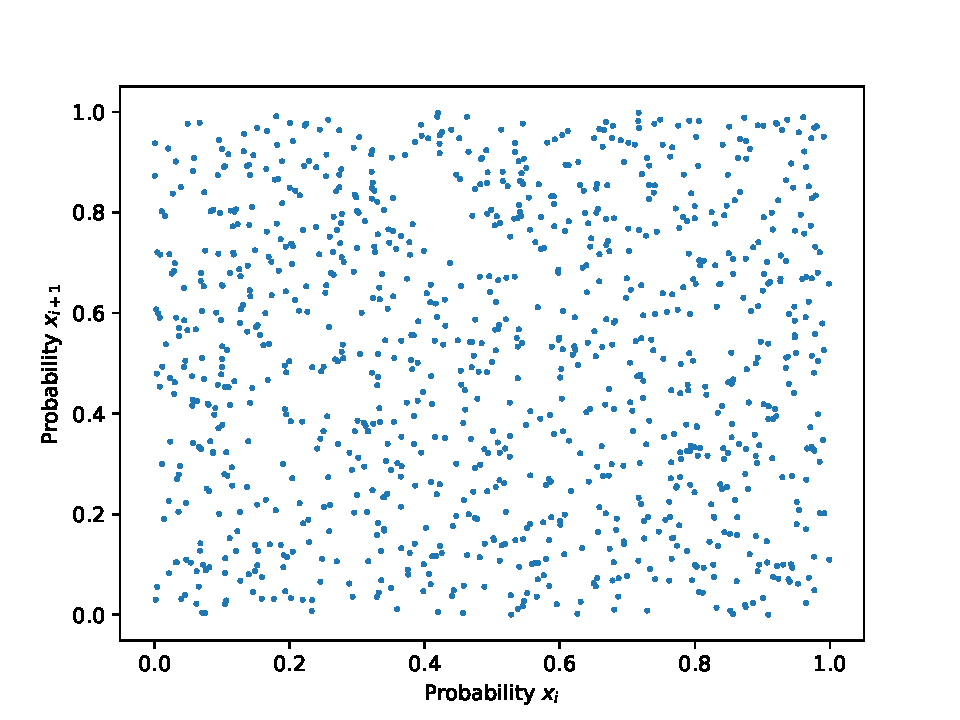
\includegraphics[width=12cm, height=7.5cm]{./Plots/1_plot_against.pdf}
\caption{TODO}
\end{figure}

\begin{figure}[!hb]
\centering
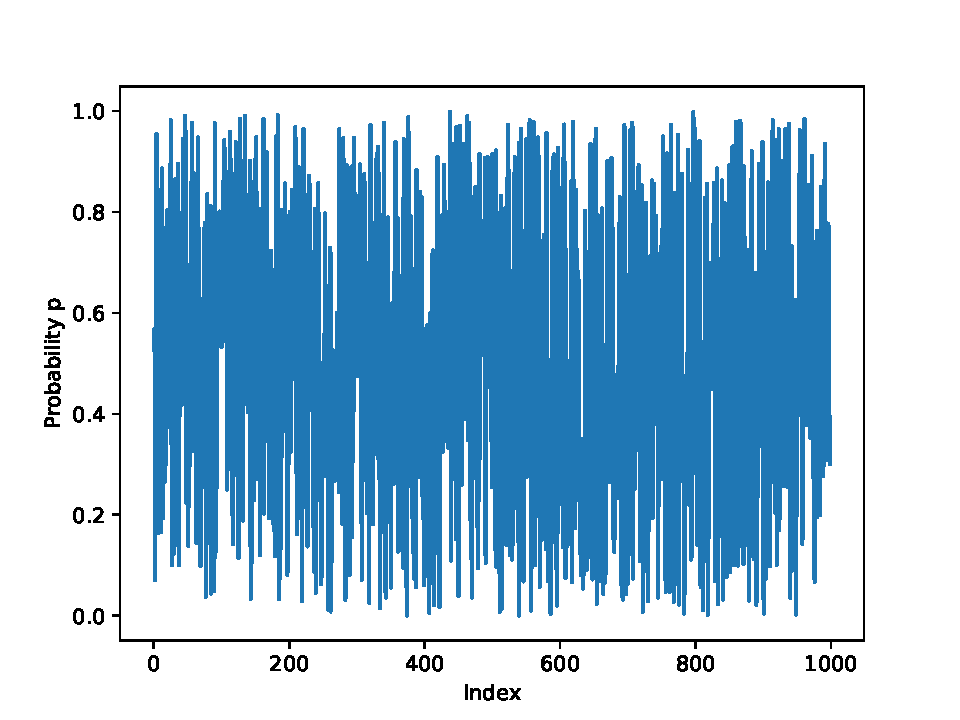
\includegraphics[width=12cm, height=7.5cm]{./Plots/1_plot_index.pdf}
\caption{TODO}
\end{figure}

\newpage
\begin{figure}[!ht]
\centering
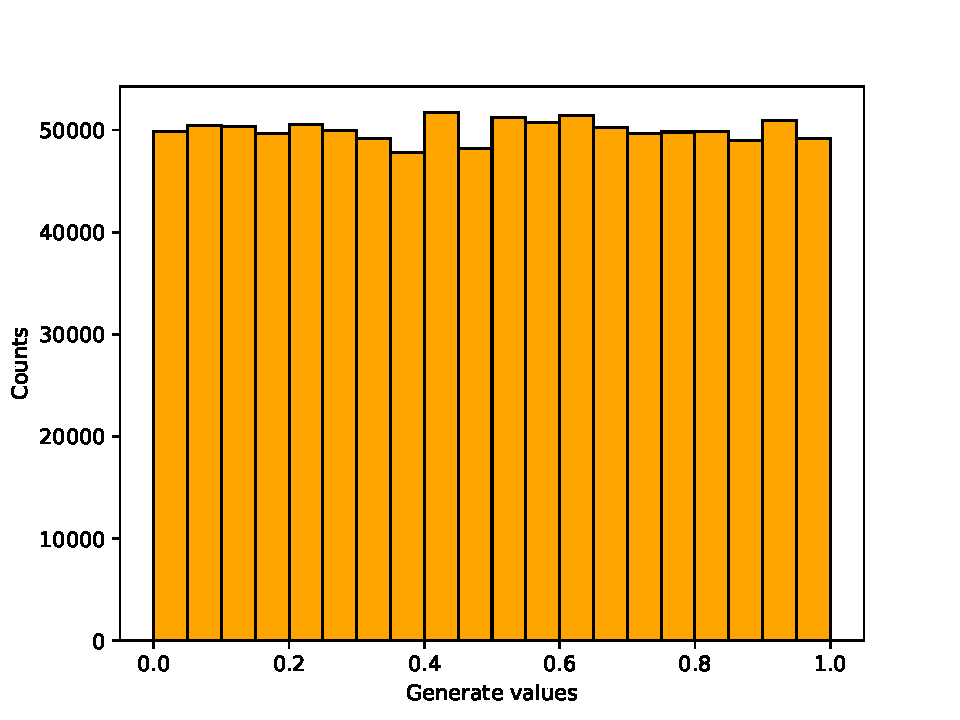
\includegraphics[width=12cm, height=7.5cm]{./Plots/1_hist_uniformnes.pdf}
\caption{TODO}
\end{figure}
\end{quote}


%\textbf{Code - helper } 
%\begin{quote}
%The code for the Poisson distribution and the factorial function.  
%\lstinputlisting[firstline=2,lastline=46]{./code/mathlib/utils.py}
%\end{quote}


%\textbf{Output}
%\begin{quote}
%The output produced by \textsf{/code/assigment1\_ a.py} 
%\lstinputlisting{./output/assigment1_a_out.txt}
%\end{quote}














\subsection*{\textbf{Question 1.b)}}
\begin{quote}

\textbf{Problem}
\begin{quote}Now use the Box-Muller method to generate 1000 normally-distributed random numbers. To check if they are following the expected Gaussian distribution, make a histogram (scaled appropriate) with the corresponding true probability distribution (normalized to integrate to 1) as line. This plot should contain the interval of -5$\sigma$ until $5\sigma$ from the theoretical probability distribution. Indicate the theoretical $1\sigma$, $2\sigma$, $3\sigma$ and $4\sigma$ interval with a line. For this plot, use $\mu =3$ and $\sigma = 2.4$ and choose bins that are appropriate.
\end{quote}

\textbf{Solution} 



\begin{quote}
The solution consists of deriving the  transformation of two i.i.d uniform variables to two i.i.d normal distributed variables with the Box-Muller method. A brief version of the derivation can be found below. The final transformation, equation \ref{EQ:boxmuller}, is  implemented in the random number generator and used to generate the plot. The final histogram is created with 20 bins and can be found on page \pageref{fig:normal}.
\\


Let $X, Y \sim G(\mu, \sigma ^2)$ be two i.i.d Gaussian distributed random variables. Their joined CDF is then given by, 
\begin{equation}
P(X \leq x_1, Y \leq y_1) =  \int_{-\infty}^{x_1} \int_{-\infty}^{y_1} G(x| \mu, \sigma^2) G(y| \mu, \sigma^2) dx dy
\end{equation}

Transforming to polar coordinates by substituting $ (x-\mu) = r \cos(\theta)$ and $ (y-\mu) = r\sin(\theta)$ yields,

\begin{align*}
P(R \leq r_1, \Theta \leq \theta_1) &= \int_0^{r_1} \int_{0}^{\theta_1} G(r\cos(\theta) \sigma + \mu| \mu, \sigma^2) G(r\sin(\theta) \sigma + \mu| \mu, \sigma^2) r dr d\theta \\
&= \frac{1}{2 \pi \sigma^2} \int_0^{r_1} \int_{0}^{\theta_1} re^{ -\frac{1}{2} \left[ \left( \frac{r\cos(\theta)}{\sigma} \right)^2  + \left( \frac{r\sin(\theta)}{\sigma} \right)^2 \right]}  dr d\theta \\
&=  \frac{1}{2 \pi \sigma^2} \int_0^{r_1} \int_{0}^{\theta_1} re^{ -\frac{r^2}{2 \sigma ^2} } dr d\theta
\end{align*}

The CDF's  for the polar coordinates are now given by, % $R$ and $\theta$ are now given by, 

\begin{align}
P(R \leq r_1) &= \frac{1}{\sigma^2} \int_{0}^{r_1}  re^{ -\frac{r^2}{2 \sigma ^2} } dr =  \int_{0}^{r_1} \frac{d}{dr} \left( -e^{ -\frac{r^2}{2 \sigma ^2}}  \right) dr = 1 - e^{- \frac{r_1^2}{2 \sigma^2}} \\
P(\Theta \leq \theta_1) &= \frac{1}{2 \pi }  \left[ -e^{-\frac{r^2}{2 \sigma^2}} \right]^{\infty}_{0} \int_{0}^{\theta_1} d\theta = \frac{\theta_1}{2\pi}
\end{align}

The CDFs can be used to convert  two uniform distributed variables to the polar coordinates of the Gaussian distributed variables. Let $U_1, U_2 \sim U(0,1)$ be two i.i.d uniform variables. From the transformation law of probability we then must have that, %The transformation law of probability then states that,

\begin{align}
P(R \leq r_1) &= P(U_1 \leq u_1) \rightarrow  1 - e^{- \frac{r_1^2}{2\sigma^2}}  = \int_{0}^{u1} du_1 = u_1 \\
P(\Theta \leq \theta) &= P(U_2 \leq u_2) \rightarrow   \frac{\theta_1}{2\pi} = \int_{0}^{u2} du_2 = u_2 
\end{align}

The transformation from the two uniform distributed variables to the polar coordinates of the Gaussian distributed variables then becomes,

\begin{align}
r_1 &=  \sqrt{-2\sigma^2 \ln(1 - u_1)} \\
\theta_1 &= 2 \pi u_2
\end{align}

Converting back to Cartesian coordinates  yields the transformation from two i.i.d uniform distributed variables to two i.i.d Gaussian distributed variables;
\begin{align}
x_1 &= r\cos(\theta) + \mu = \sqrt{-2\sigma^2 \ln(1 - u_1)} \cos( 2 \pi u_2 ) + \mu \\
y_1 &= r\sin(\theta) + \mu = \sqrt{-2\sigma^2 \ln(1 - u_1)} \sin( 2 \pi u_2 ) + \mu
\label{EQ:boxmuller}
\end{align}
\\
\\
These above transformation are implemented in  the random number generator (see page \pageref{CODE:RNG}).  The code for the generation of the plot and the created plot can be found below. The code that generates the plot makes besides the RNG use of a function for the normal distribution in the file \texttt{./Code/mathlib/statistics.py}. This file is treated as a shared module and can be found on page 22. The called function, \texttt{normal}, can be found on line 227 in this file.


\end{quote}

\textbf{Code - Plots}

\begin{quote}
The code for generating the plots. The imports are again not explicit shown, but can be found on page 19. The shared modules can be found on pages 19 and 22. 


\lstinputlisting[firstline=68,lastline=122]{./Code/assigment_1.py}
\end{quote}


\textbf{Code - Output plot(s)}
\vspace*{-0.5cm}
\begin{quote}
\begin{figure}[!hb]
\centering
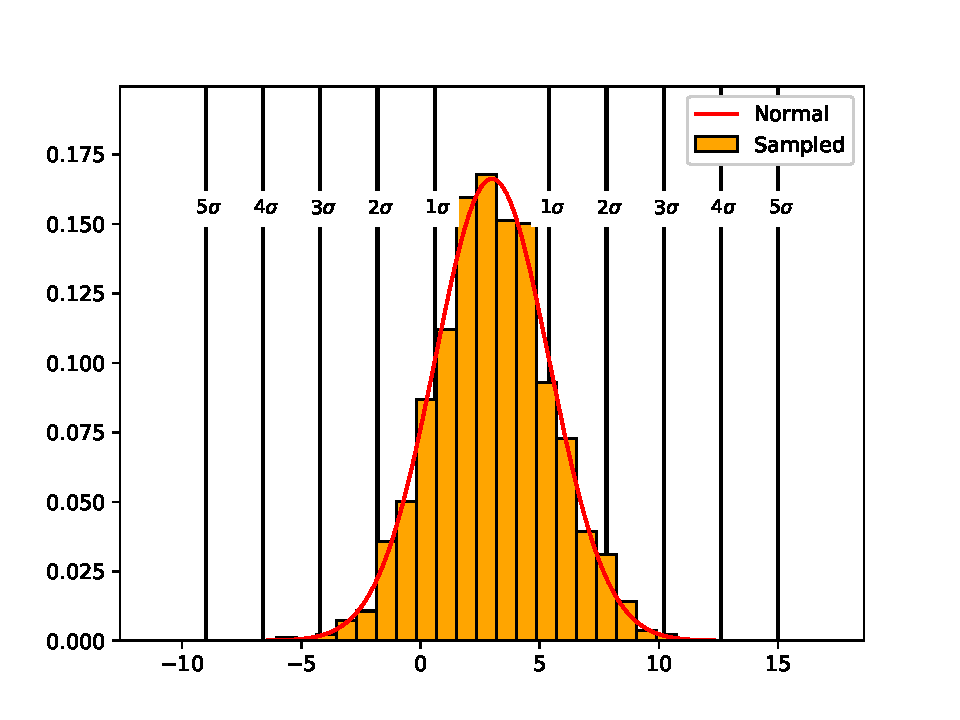
\includegraphics[width=13cm, height=7.0cm]{./Plots/1_hist_gaussian.pdf}
\caption{A histogram of the 1000 random normal distributed variables generated with the box muller method for $\mu = 3$ and $\sigma = 2.4$  (orange). The red line is the true normal distribution.  The histogram appears to approximate the distribution quite well, but displays small deviations. The bin left of the peak (the highest bin) is larger than it should be. The first bins right of the peak is smaller than it should be and the second bin right of the peak is to high.  The histogram does however still appear to be acceptable by eye. A statistical test is of course better to determine whether the histogram would truly be acceptable or not.}
\label{fig:normal}
\end{figure}
\end{quote}
\end{quote}

%\textbf{Code - output } 
%\begin{quote}
% The code that produces the output.
%\lstinputlisting{./code/assigment1_a.py}
%\end{quote}

%\textbf{Code - helper } 
%\begin{quote}
%The code for the Poisson distribution and the factorial function.  
%\lstinputlisting[firstline=2,lastline=46]{./code/mathlib/utils.py}
%\end{quote}


%\textbf{Output}
%\begin{quote}
%The output produced by \textsf{/code/assigment1\_ a.py} 
%\lstinputlisting{./output/assigment1_a_out.txt}
%\end{quote}













\subsection*{\textbf{Question 1.c}}
\begin{quote}

\textbf{Problem}
\begin{quote}
Write a code that can do the KS-test on the your function to determine if it is consistent with a normal distribution. For this, use $\mu = 0$ and $\sigma = 1$. Make a plot of the probability that your Gaussian random number generator is consistent with Gaussian distributed random numbers, start with 10 random numbers and use in your plot a spacing of 0.1 dex until you have calculated it for $10^5$ random numbers on the x-axis. Compare your algorithm with the KS-test function from \texttt{scipy, scipy.stats.kstest} by making an other plot with the result from your KS-test and the KS-test from scipy.
\end{quote}

\textbf{Solution} 
\begin{quote}
The implementation of the KS-test is in general straight forwards. There are however two points of interest that needs to be discussed. The first point is the implementation of the CDF for the KS-statistic and the second point is the implementation of the CDF for the normal distribution.
\\

\textbf{(1) CDF KS-statistic }
\begin{quote}
The p-value produced by the KS-tests requires the evaluation of the CDF for the KS-test statistic,
\begin{equation}
P_{KS}(z) = \frac{2\sqrt{\pi}}{z} \sum_{j=1}^{\infty} \exp\left(- \frac{(2j-1)^2+\pi^2}{8z^2} \right)
\end{equation}

This infinite sum needs to be numerically approximated in order to perform the KS-test. The chosen approximation in the implementation of the KS-test for  the sum is taken from the book \textit{Numerical Recipes - The art of Scientific Computation, 3d edition}, %... who states that the sum can be approximated by, % approximation can according to .. be approximated by, 
\begin{equation}
P_{KS}(z) \approx
\begin{cases}
\frac{\sqrt{2 \pi}}{z} \left[ \left( e^{-\pi^2/(8z^2)} \right)+^{9} + \left( e^{-\pi^2/(8z^2)} \right) \left( e^{-\pi^2/(8z^2)} \right)^{25} \right] &\quad \text{for $ z < 1.18$}\\
1 -2 \left[ \left(e^{-2z^2}\right) - \left(e^{-2z^2}\right)^4 + \left(e^{-2z^2}\right)^9 \right]  &\quad \text{for $ z >= 1.18$}
\end{cases}
\end{equation}
\end{quote}

\textbf{(2) CDF normal distribution}
\begin{quote}
The CDF of the normal distribution is needed in order to perform the KS-test under the null hypothesis that the data follows a normal distribution. The CDF of the normal distribution can in general be written as,
\begin{equation}
\Phi\left( \frac{x- \mu}{\sigma}\right) = \frac{1}{2} \left[ 1 + \text{erf} \left( \frac{x - \mu}{\sigma\sqrt{2}} \right) \right]
\end{equation}

where the erf is given by,
\begin{equation}
\text{erf}(x)  \frac{2}{\sqrt{\pi}} \int_0^{x} e^{-t^2} dt
\end{equation}

The integral of the erf function lacks a closed form and therefore also needs to be numerically approximated. The chosen approximation is taken from \textit{Abramowitz and Stegun},

\begin{equation}
\text{erf}(x) \approx 1- (a_1t+a_2t^2 + ... + a_5t^5)e^{-x^2} \text{x} \quad t = \frac{1}{1+px}
\end{equation}

where $p  =0.3275911$, $a_1 =  0.254829592$, $a_2 = -0.284496736$, $a_3 = 1.421413741$, $a_4 =  -1.453152027$, $a_5 = 1.061405429$.
\end{quote}

The KS-test and the CDF are implemented with these approximations. The code for the KS-test and the CDF  is located in the file \texttt{./Code/mathlib/statistics.py} at page \pageref{CODE:Statistics}, as this file is threaded as a shared module. The KS-test does require an sorting algorithm, this algorithm is implemented in the file \texttt{./Code/matlib/sorting} and can be found on page \pageref{CODE:sorting}. 
 The code for the generation of the plots and plots are displayed below.  
\end{quote}

\newpage
\textbf{Code - Plots}

\begin{quote}
The code for generating the two plots. The imports for this file are not explicit shown, but can be found on page \pageref{CODE:MAIN1}.
\lstinputlisting[firstline=125,lastline=180]{./Code/assigment_1.py}
\end{quote}
\newpage

\textbf{Code - Output plot(s)}
\begin{quote}
\begin{figure}[!ht]
\centering
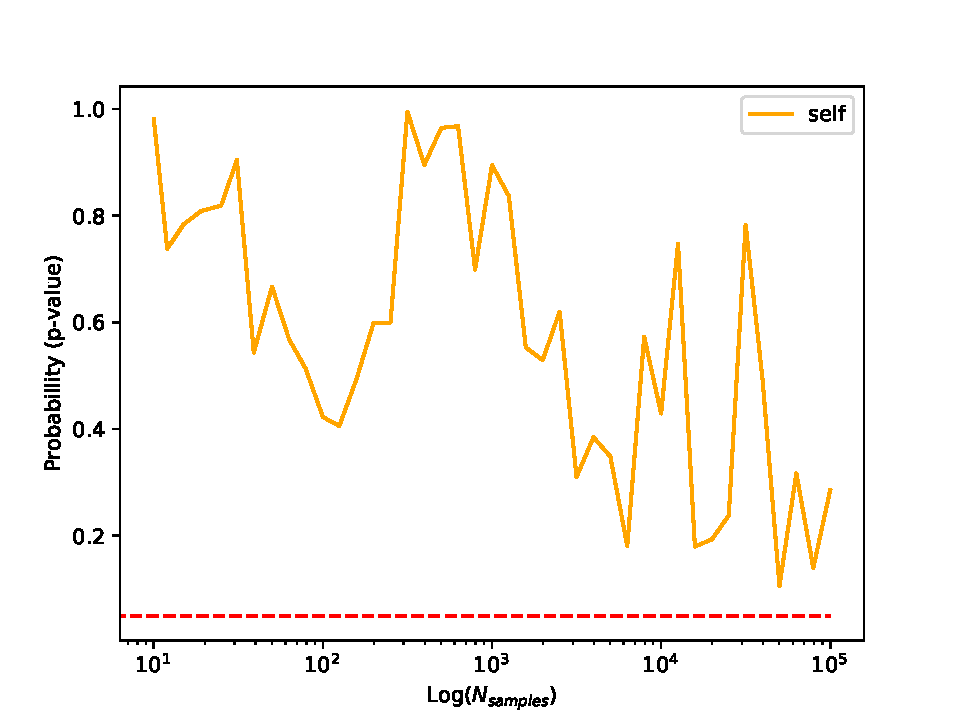
\includegraphics[width=12cm, height=7.5cm]{./Plots/1_plot_ks_test_self.pdf}
\caption{The P-value produced by the KS-test against the number of samples on which the KS-test is performed for the self written RNG. The red line indicates the line of $ p = 0.05$. A point \textbf{below} the line would suggests that there is enough statistical evidence to reject the (null) hypothesis that the data is normal distributed. The plot shows that the RNG always passes KS-test up to atleast $10^5$ samples. The p-value  does however appear to drop for a large number of samples and might even drop further when more samples are used. The drop suggests again that the RNG is likely not perfect.}
\end{figure}

\begin{figure}[!hb]
\centering
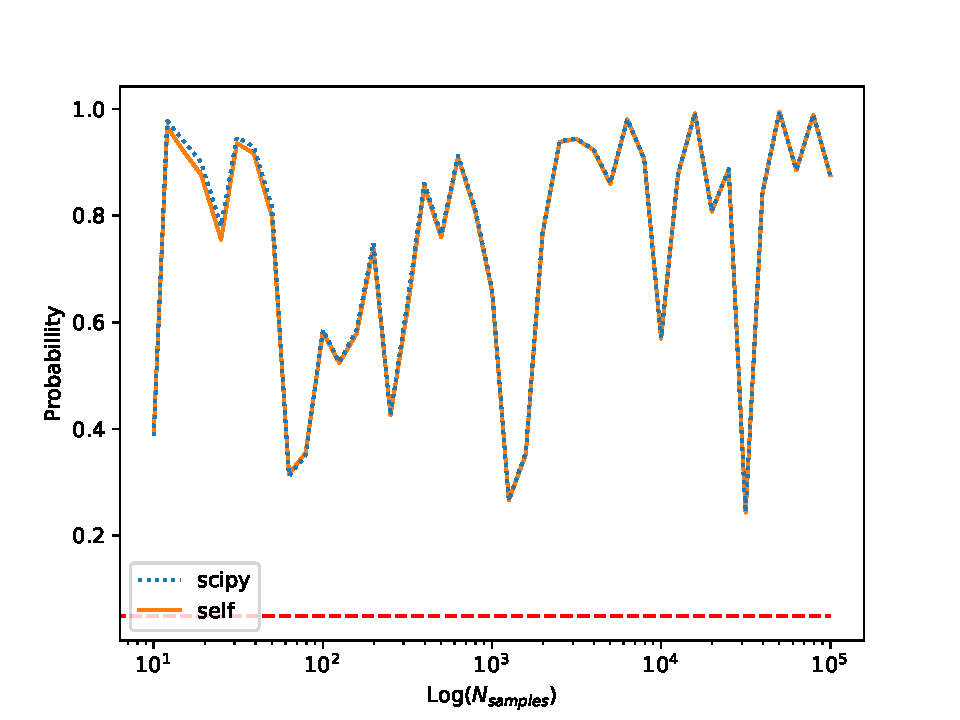
\includegraphics[width=12cm, height=7.5cm]{./Plots/1_plot_ks_test_self_scipy.pdf}
\caption{The P-value produced by the KS-test against the number of samples on which the KS-test is performed for the self written RNG. The red line indicates the line of $ p = 0.05$. The orange line is the self written implementation of the KS-test and the blue line is the scipy version.  A point \textbf{below} the red line would suggests that there is enough statistical evidence to reject the (null) hypothesis that the data is normal distributed. The self written KS-test is  close to the scipy version, but shows (small) deviations at small sample sizes (for example at $N_{samples} = 10$ or $N_{samples} = 200$).  The self written implementation always has the same shape as the scipy version, even at the deviations. The exact cause for the deviations are unknown, but are likely the result of an approximation that scipy makes that the self written implementation doesn't make. (This is not confirmed by looking at the scipy code.) }
\end{figure}
\end{quote}

\end{quote}



%\textbf{Code - output } 
%\begin{quote}
% The code that produces the output.
%\lstinputlisting{./code/assigment1_a.py}
%\end{quote}

%\textbf{Code - helper } 
%\begin{quote}
%The code for the Poisson distribution and the factorial function.  
%\lstinputlisting[firstline=2,lastline=46]{./code/mathlib/utils.py}
%\end{quote}


%\textbf{Output}
%\begin{quote}
%The output produced by \textsf{/code/assigment1\_ a.py} 
%\lstinputlisting{./output/assigment1_a_out.txt}
%\end{quote}












\subsection*{\textbf{Question 1.d)}}
\begin{quote}

\textbf{Problem}
\begin{quote}
Write a code that does the Kuiper’s test on your random numbers (see tutorial
8) and make the same plot as for the KS-test.
\end{quote}

\textbf{Solution} 
\begin{quote}
The implementation of the Kuiper test does require a numerical approximation of the CDF for the kuiper statistics. The CDF of the kuiper staistic is given by, 
\begin{equation}
P_{kuiper}( \lambda) =  1 - 2  \sum_{j=1}^{\infty} (4j^2 \lambda^2-1) e^{-2j^2 \lambda^2 }
\end{equation}

The sum is in the above expression negligible compared to the machine error if $\lambda < 0.4$. In this case the numerically approximation thus consist of returning 1.  If $\lambda > 0.4$ then the sum is approximated by calculating the first 100 terms of the sum. This should be more than enough for the sum to converge. \footnote{Actually, less terms are enough. The evaluation of the sum could therefore stop early by checking for a required precision. } 

The Kuiper-test and the CDF are implemented in the shared module \texttt{./Code/mathlib/statistics.py} that can be found on page 22. The code that creates the plots and the plots can be found below.  The code does make use of \textbf{astropy} to compare the self written implementation of the Kuiper-test with the implementation of astropy. 
\end{quote}

\textbf{Code - Plots}

\begin{quote}
The code for generating the two plots. The imports are not explicit shown but can be shown on page 19. 
\lstinputlisting[firstline=182,lastline=235]{./Code/assigment_1.py}
\end{quote}

\textbf{Code - Output plot(s)}
\begin{quote}
\begin{figure}[!ht]
\centering
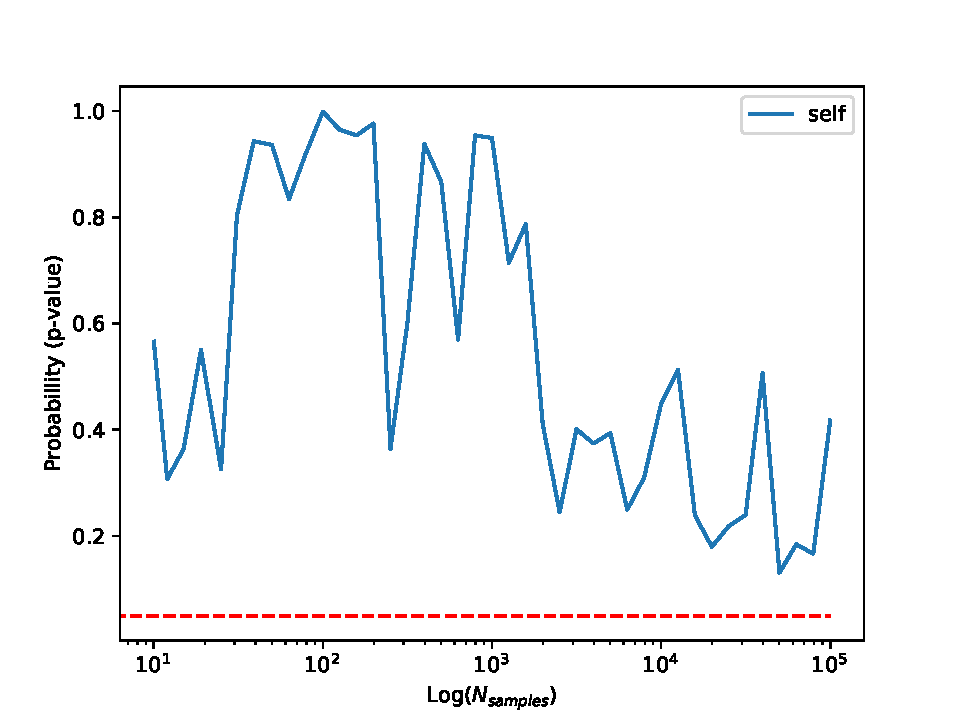
\includegraphics[width=12cm, height=7.5cm]{./Plots/1_plot_kuiper_test_self.pdf}
\caption{The P-value produced by the Kuiper-test against the number of samples on which the kuiper-test is performed for the self written RNG. The red line indicates the line of $ p = 0.05$. A point \textbf{below} there  line would suggests that there is enough statistical evidence to reject the (null) hypothesis that the data is normal distributed. The plot shows that the RNG always passes Kuiper test. It can however be seen that the p-value drops for larger sample size, similar as what happens by the KS-test. This might, as mentioned before, indicate that there is an flaw in the random number generator.}
\end{figure}
\newpage
\begin{figure}[!hb]
\centering
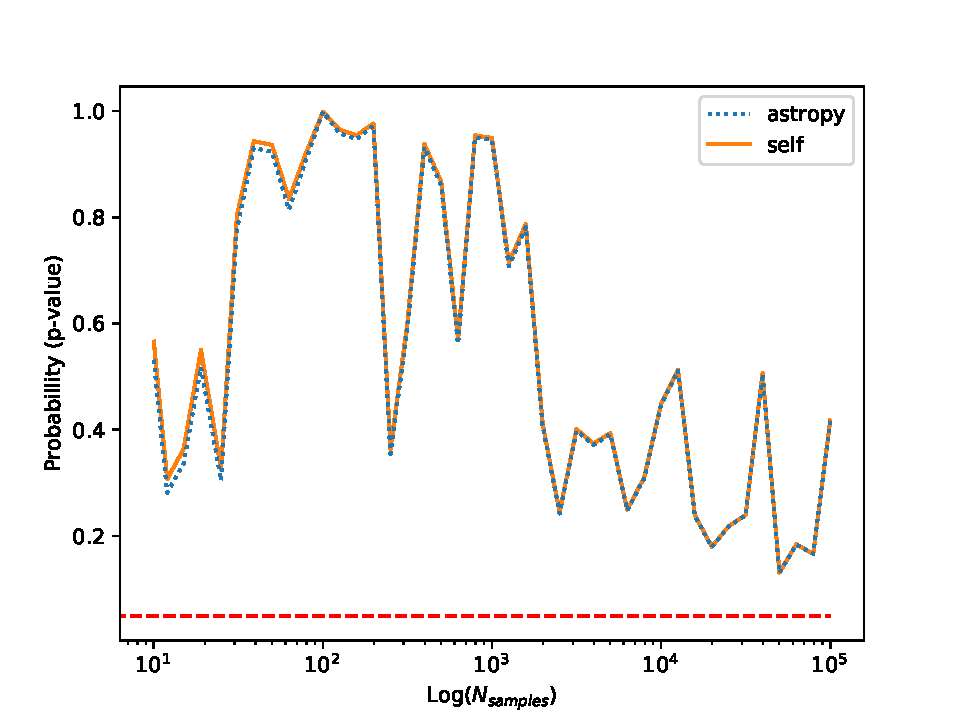
\includegraphics[width=12cm, height=7.5cm]{./Plots/1_plot_kuiper_test_self_astropy.pdf}
\caption{The P-value produced by the kuiper test against the number of samples on which the kuiper-test is performed for the self written RNG. The red line indicates the line of $ p = 0.05$. A point \textbf{below} there  line would suggests that there is enough statistical evidence to reject the (null) hypothesis that the data is normal distributed. The plot shows that the self written implementation has (small) deviations from the astropy implementation at small sample sizes. This is similar to the situation with the KS-test and might be caused by an approximation made in astropy.   }
\end{figure}

\end{quote}
\end{quote}
















\subsection*{\textbf{Question 1.e)}}
\begin{quote}

\textbf{Problem}
\begin{quote}
Download the dataset. The dataset contains 10 sets of random numbers. Compare these 10 sets with your Gaussian pseudo random numbers and make the plot of the probabilities as in either of the previous two exercises (your choice). Which random number arrays is/are consistent with a Gaussian random numbers with $\sigma = 1$ and $\mu = 0$
\end{quote}

\textbf{Solution} 
\begin{quote}
The distributions are compared by performing the KS-test 2 (2 sample distributions). The KS-test 2 has to be applied to 10 columns. The random numbers that are compared with the column data are as result only generated once (i.e each column is  compared with the same random numbers). This was done to save computation time.  The code that contains the implementation of the ks-test 2 can be found on page 22.  The code that generates the plots and the generated plots can be found below.
\\
\\
The plots show that there is only one column which might be\footnote{A p-value only shows statistical evidence against the null hypothesis, it isn't a measure of how good the null hypothesis is.} a normal distribution with $\sigma = 1$ and $\mu = 0$. This is column 4 (index 3, see figure 12 on page 15). In all other plots the p-value drops and stays below $ p = 0.05$ when including all samples, which indicates that their is enough statistical evidence to reject the hypothesis that they follow a normal distribution with $\sigma = 1$ and $\mu = 0$. 

\end{quote}
\newpage

\textbf{Code - Plots}

\begin{quote}
The code for generating the 10 plots. 
\lstinputlisting[firstline=236,lastline=290]{./Code/assigment_1.py}
\end{quote}
\newpage


\textbf{Code - Output plot(s)} \\
\textbf{Note:} Expect very similar captions for the upcoming 10 plots.
\begin{quote}
\begin{figure}[!ht]
\centering
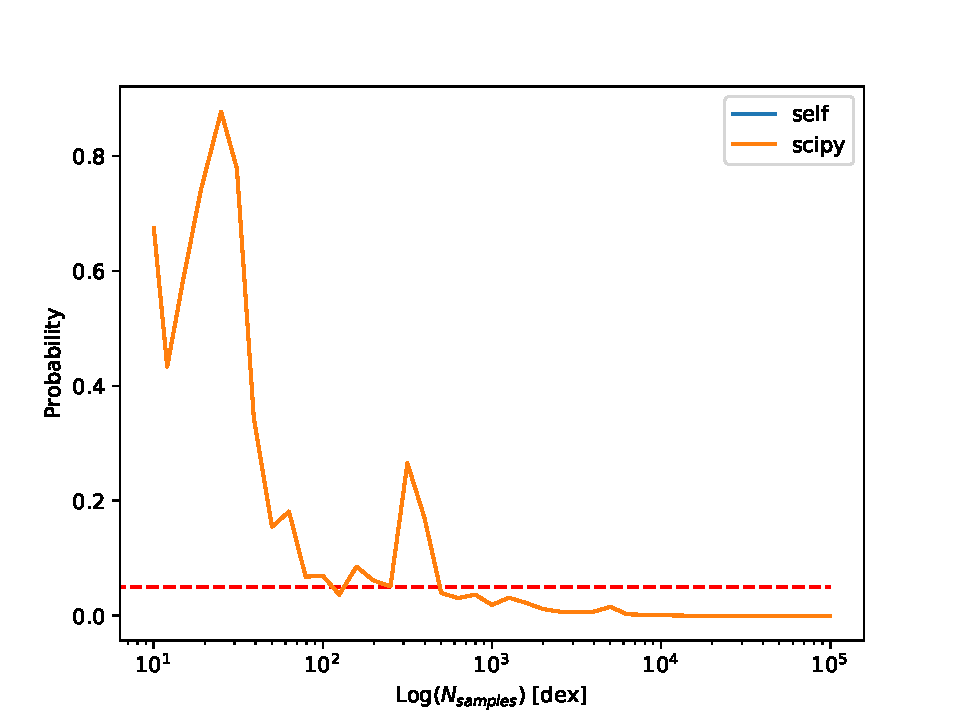
\includegraphics[width=14cm, height=8cm]{./Plots/1e_plot_column_0.pdf}
\caption{The P-value produced by performing the KS-test2 for a normal distribution with $\mu = 0$ and $\sigma = 1$ on the \textbf{first} column.  The red line indicates the line of $ p = 0.05$. A point \textbf{below} there  line would suggests that there is enough statistical evidence to reject the (null) hypothesis that the data is normal distributed. The plot shows that the p-value drops below 0.05 when including all samples. There is thus enough statistical evidence to reject the hypothesis that this column is normal distributed with $\mu = 0$ and $\sigma = 1$.}
\end{figure}

\begin{figure}[!ht]
\centering
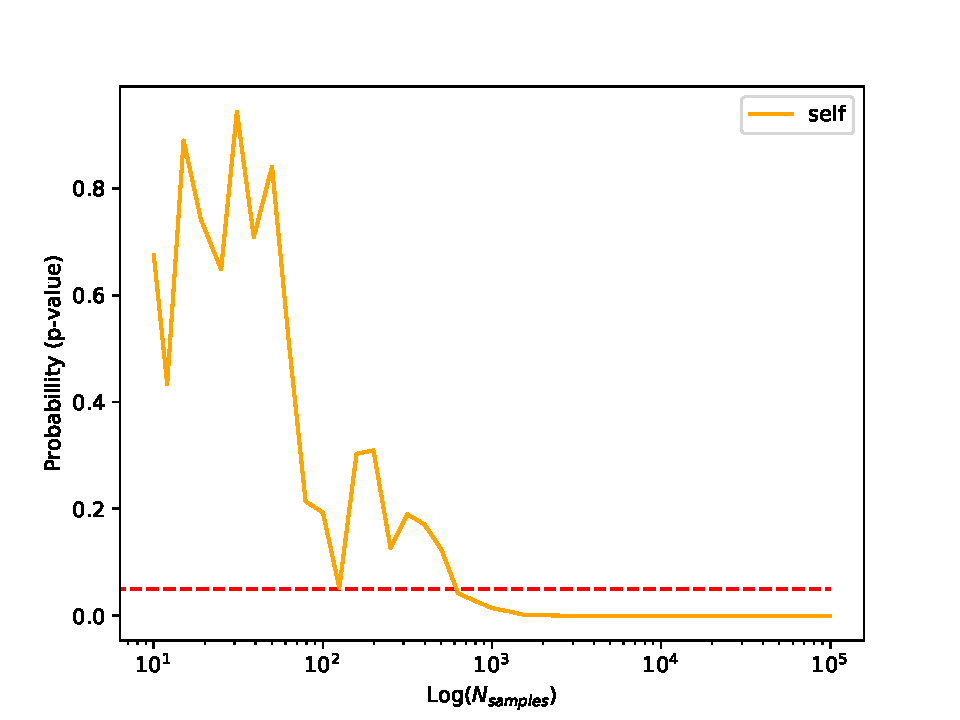
\includegraphics[width=14cm, height=8cm]{./Plots/1e_plot_column_1.pdf}
\caption{The P-value produced by performing the KS-test2 for a normal distribution with $\mu = 0$ and $\sigma = 1$ on the \textbf{second} column.  The red line indicates the line of $ p = 0.05$. A point \textbf{below} there  line would suggests that there is enough statistical evidence to reject the (null) hypothesis that the data is normal distributed. The plot shows that the p-value drops below 0.05 when including all samples. There is thus enough statistical evidence to \textbf{reject} the hypothesis that this column is normal distributed with $\mu = 0$ and $\sigma = 1$.}
\end{figure}
\newpage

\begin{figure}[!ht]
\centering
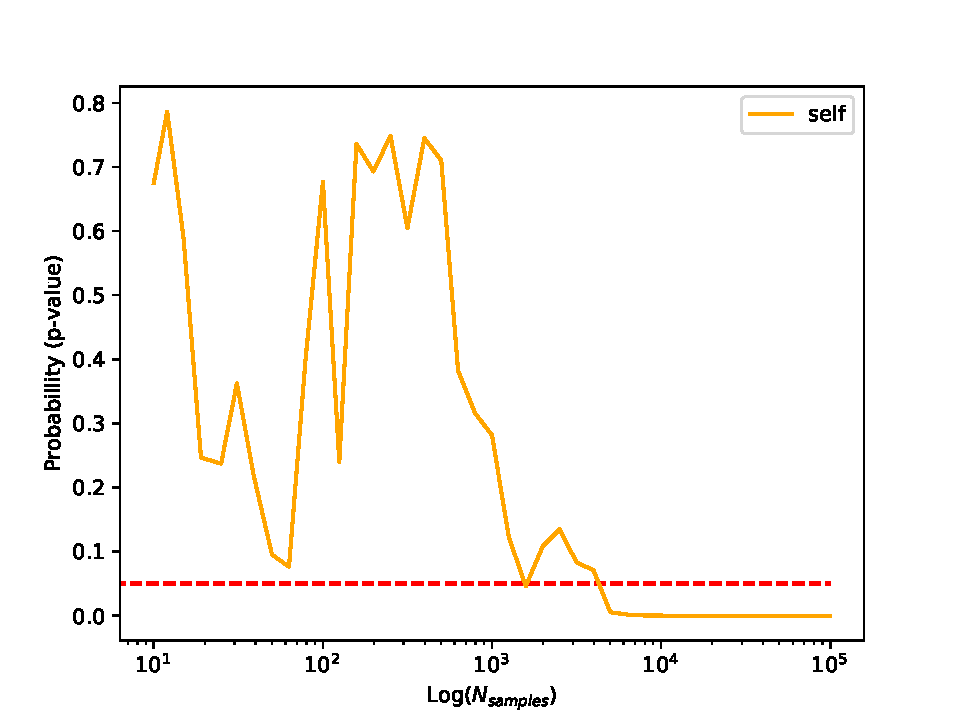
\includegraphics[width=14cm, height=8.5cm]{./Plots/1e_plot_column_2.pdf}
\caption{The P-value produced by performing the KS-test2 for a normal distribution with $\mu = 0$ and $\sigma = 1$ on the \textbf{third} column.  The red line indicates the line of $ p = 0.05$. A point \textbf{below} there  line would suggests that there is enough statistical evidence to reject the (null) hypothesis that the data is normal distributed. The plot shows that the p-value drops below 0.05 when including all samples. There is thus enough statistical evidence to \textbf{reject} the hypothesis that this column is normal distributed with $\mu = 0$ and $\sigma = 1$.}
\end{figure}

\begin{figure}[!ht]
\centering
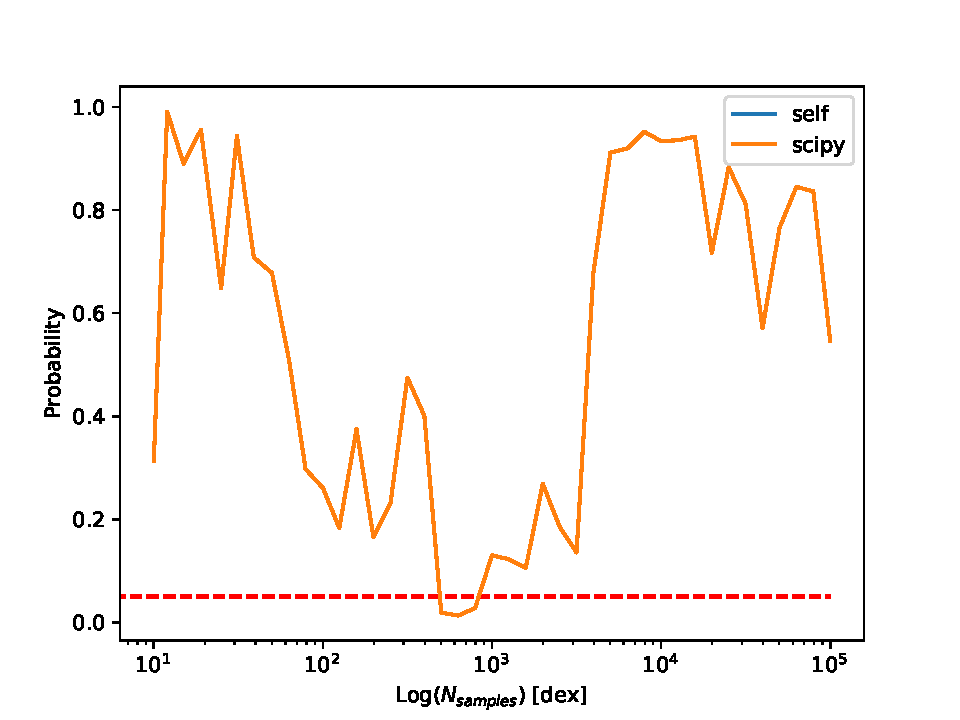
\includegraphics[width=14cm, height=8.5cm]{./Plots/1e_plot_column_3.pdf}
\label{FIG:Good}
\caption{The P-value produced by performing the KS-test2 for a normal distribution with $\mu = 0$ and $\sigma = 1$ on the \textbf{fourth} column.  The red line indicates the line of $ p = 0.05$. A point \textbf{below} there  line would suggests that there is enough statistical evidence to \textbf{reject} the (null) hypothesis that the data is normal distributed. The plot shows that the p-value drops below 0.05 only between $500-1000$ samples. In all other cases it passes the KS-test. The most important point in this plot is the p-value when all samples are included. It can be clearly seen that this point isn't below the red line. The plot therefore suggests that the given c olumn might( see footnote 2 on page 12) be a Gaussian with $\mu = 0$ and $\sigma =1$.  }
\end{figure}
\newpage

\begin{figure}[!ht]
\centering
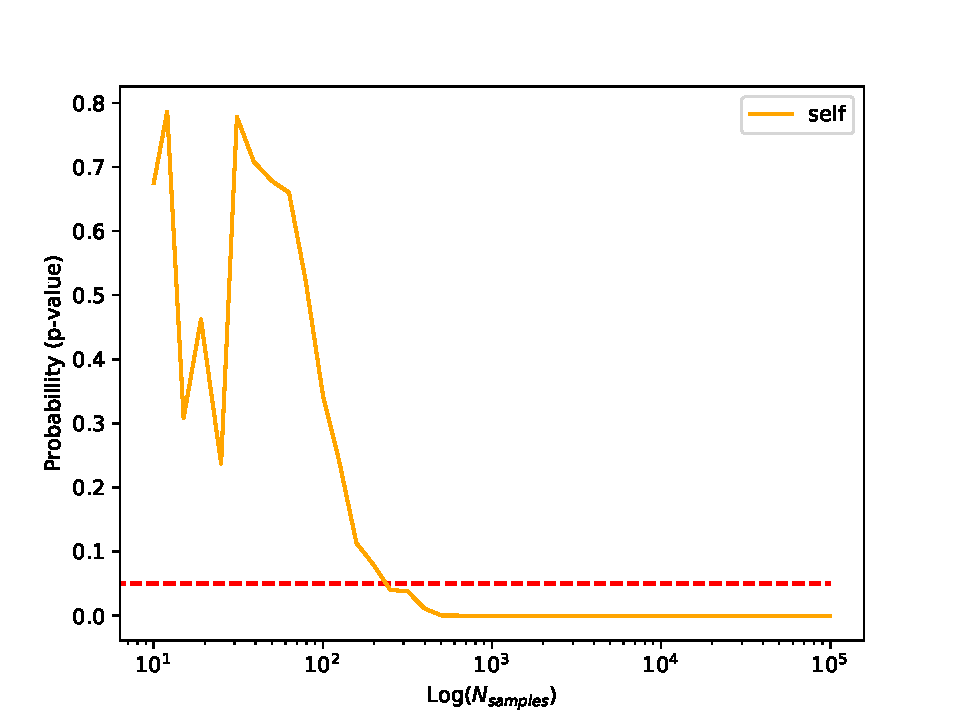
\includegraphics[width=14cm, height=8.5cm]{./Plots/1e_plot_column_4.pdf}
\caption{The P-value produced by performing the KS-test2 for a normal distribution with $\mu = 0$ and $\sigma = 1$ on the \textbf{fifth} column.  The red line indicates the line of $ p = 0.05$. A point \textbf{below} there  line would suggests that there is enough statistical evidence to reject the (null) hypothesis that the data is normal distributed. The plot shows that the p-value drops below 0.05 when including all samples. There is thus enough statistical evidence to reject the hypothesis that this column is normal distributed with $\mu = 0$ and $\sigma = 1$.}
\end{figure}


\begin{figure}[!ht]
\centering
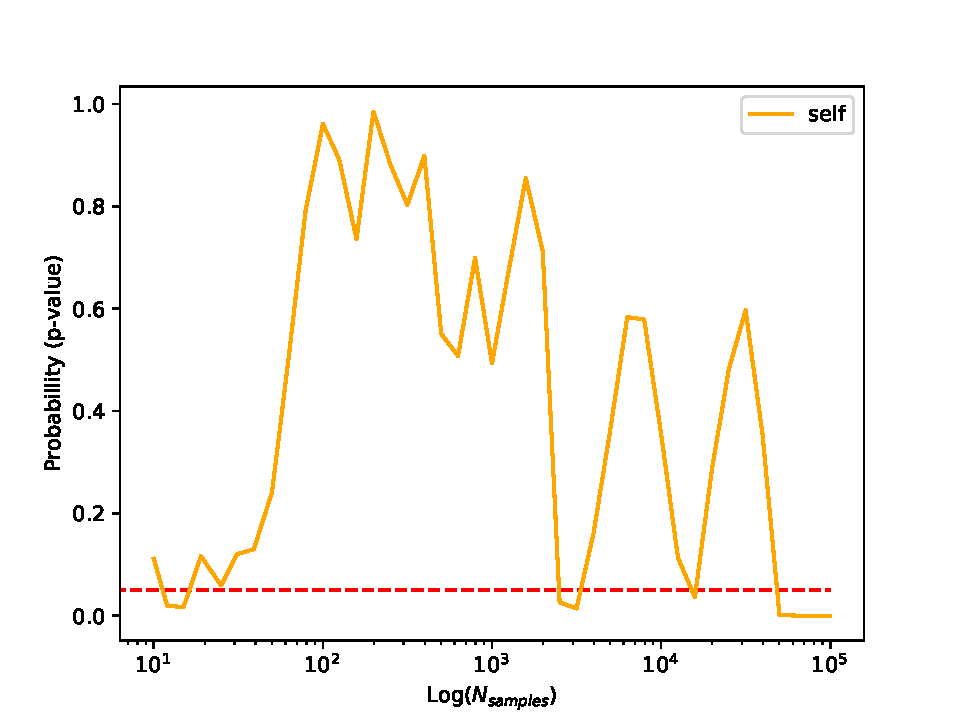
\includegraphics[width=14cm, height=8.5cm]{./Plots/1e_plot_column_5.pdf}
\caption{The P-value produced by performing the KS-test2 for a normal distribution with $\mu = 0$ and $\sigma = 1$ on the \textbf{sixth} column.  The red line indicates the line of $ p = 0.05$. A point \textbf{below} there  line would suggests that there is enough statistical evidence to reject the (null) hypothesis that the data is normal distributed. The plot shows that the p-value drops below 0.05 and stays there when including more than halve of the samples. The most important part of the figure is the part that includes most samples. There is thus enough statistical evidence to reject the hypothesis that this column is normal distributed with $\mu = 0$ and $\sigma = 1$.}
\end{figure}

\newpage

\begin{figure}[!ht]
\centering
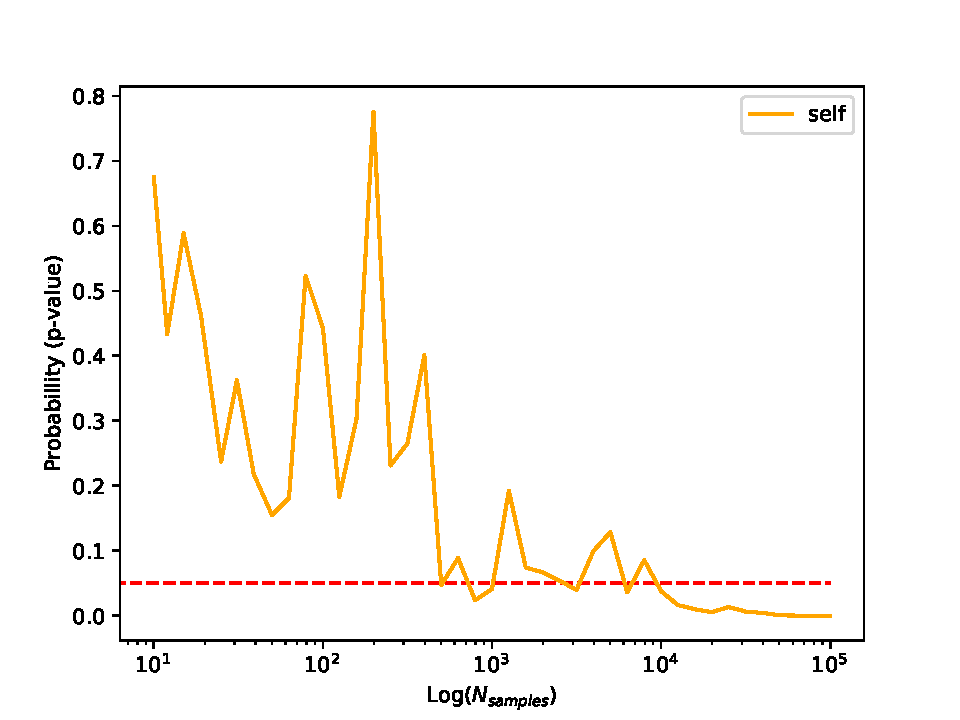
\includegraphics[width=14cm, height=8.5cm]{./Plots/1e_plot_column_6.pdf}
\caption{The P-value produced by performing the KS-test2 for a normal distribution with $\mu = 0$ and $\sigma = 1$ on the \textbf{seventh} column.  The red line indicates the line of $ p = 0.05$. A point \textbf{below} there  line would suggests that there is enough statistical evidence to reject the (null) hypothesis that the data is normal distributed. The plot shows that the p-value drops below 0.05 when including all samples. There is thus enough statistical evidence to reject the hypothesis that this column is normal distributed with $\mu = 0$ and $\sigma = 1$.}
\end{figure}


\begin{figure}[!ht]
\centering
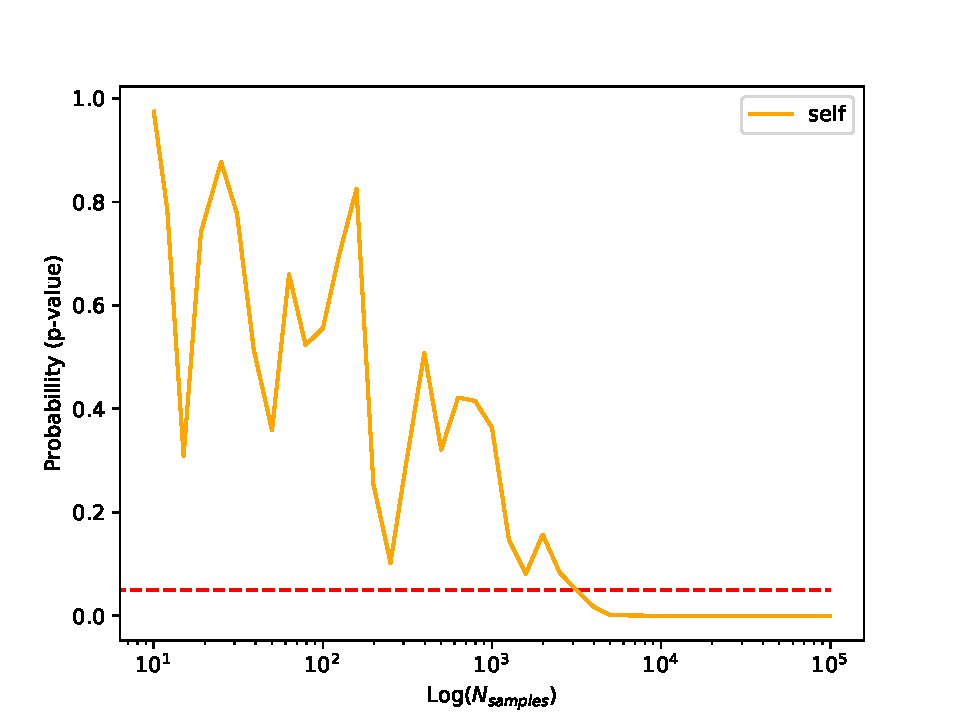
\includegraphics[width=14cm, height=8.5cm]{./Plots/1e_plot_column_7.pdf}
\caption{The P-value produced by performing the KS-test2 for a normal distribution with $\mu = 0$ and $\sigma = 1$ on the \textbf{eight} column.  The red line indicates the line of $ p = 0.05$. A point \textbf{below} there  line would suggests that there is enough statistical evidence to reject the (null) hypothesis that the data is normal distributed. The plot shows that the p-value drops below 0.05 when including all samples. There is thus enough statistical evidence to reject the hypothesis that this column is normal distributed with $\mu = 0$ and $\sigma = 1$.}
\end{figure}

\newpage

\begin{figure}[!ht]
\centering
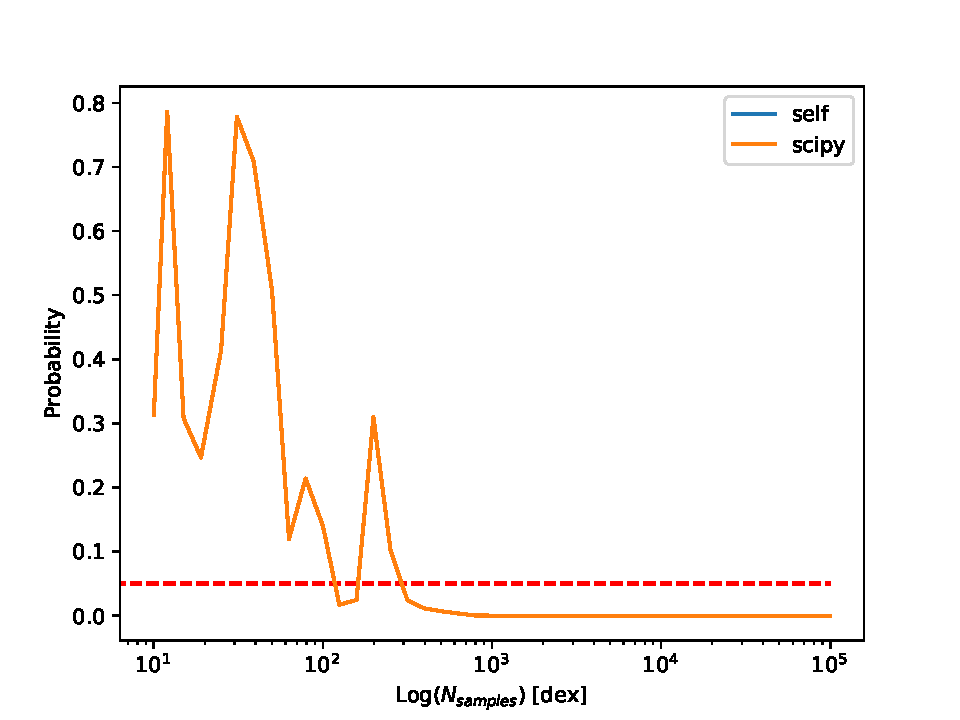
\includegraphics[width=14cm, height=8.5cm]{./Plots/1e_plot_column_8.pdf}
\caption{The P-value produced by performing the KS-test2 for a normal distribution with $\mu = 0$ and $\sigma = 1$ on the \textbf{ninth} column.  The red line indicates the line of $ p = 0.05$. A point \textbf{below} there  line would suggests that there is enough statistical evidence to reject the (null) hypothesis that the data is normal distributed. The plot shows that the p-value drops below 0.05 when including all samples. There is thus enough statistical evidence to reject the hypothesis that this column is normal distributed with $\mu = 0$ and $\sigma = 1$.}
\end{figure}

\begin{figure}[!ht]
\centering
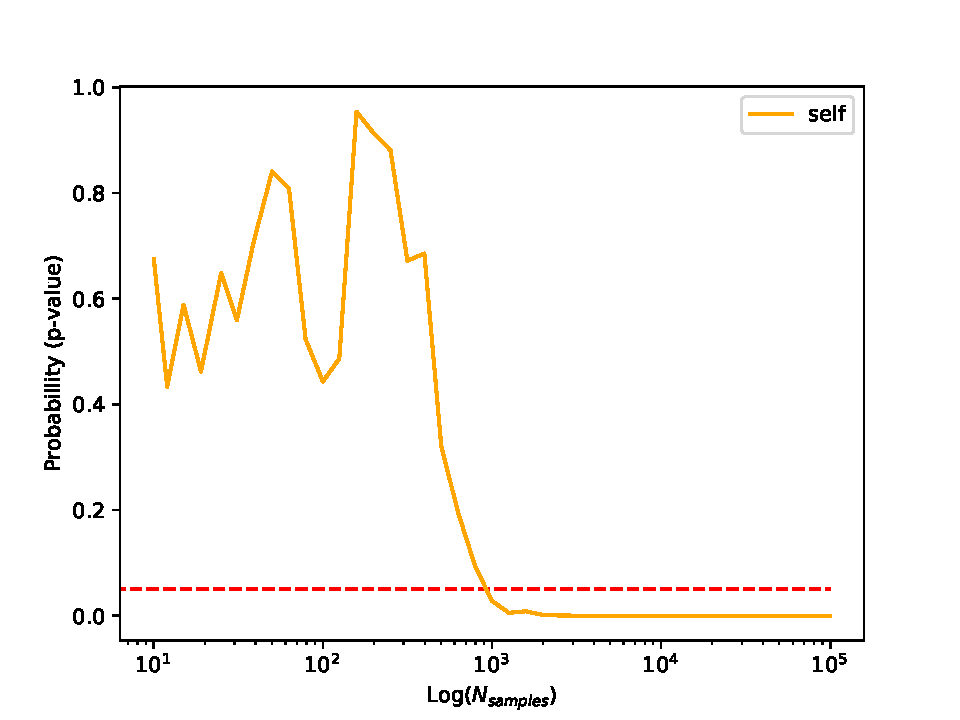
\includegraphics[width=14cm, height=8.5cm]{./Plots/1e_plot_column_9.pdf}
\caption{The P-value produced by performing the KS-test2 for a normal distribution with $\mu = 0$ and $\sigma = 1$ on the \textbf{tenth} column.  The red line indicates the line of $ p = 0.05$. A point \textbf{below} there  line would suggests that there is enough statistical evidence to reject the (null) hypothesis that the data is normal distributed. The plot shows that the p-value drops below 0.05 when including all samples. There is thus enough statistical evidence to reject the hypothesis that this column is normal distributed with $\mu = 0$ and $\sigma = 1$.}
\end{figure}
\end{quote}



\end{quote}

\newpage

%\textbf{Code - output } 
%\begin{quote}
% The code that produces the output.
%\lstinputlisting{./code/assigment1_a.py}
%\end{quote}

%\textbf{Code - helper } 
%\begin{quote}
%The code for the Poisson distribution and the factorial function.  
%\lstinputlisting[firstline=2,lastline=46]{./code/mathlib/utils.py}
%\end{quote}


%\textbf{Output}
%\begin{quote}
%The output produced by \textsf{/code/assigment1\_ a.py} 
%\lstinputlisting{./output/assigment1_a_out.txt}
%\end{quote}
\newpage













\subsection*{\textbf{Question 1- Summary}}
\begin{quote}

\textbf{Summary}
\begin{quote}
The current sub-section contains the summary of the code used for assignment 1. This includes the file  containing all sub-questions and all used shared modules. 
\end{quote}


\textbf{Code - Assignment}

\begin{quote}
The code of the file that executes the sub-questions. The code presented below only consists of the part that has not jet been shown in the subquestions.  This part consists of the initialization of the random number generator (1.a) and the used imports. 
\label{CODE:MAIN1}
\lstinputlisting[firstline=0,lastline=18]{./Code/assigment_1.py}
\end{quote}

\textbf{Code - Random Number Generator} \\
\begin{quote}
The code for the random number generator.
\label{CODE:RNG}
\lstinputlisting{./Code/mathlib/random.py}
\end{quote}

\textbf{Code - Statistical functions} \\

\begin{quote}
The code that containing all statistical functions that where needed for the sub-questions. The imported sorting module used by this piece of code can be found on page 26. 
\label{CODE:Statistics}

\lstinputlisting{./Code/mathlib/statistics.py}
\end{quote}

\textbf{Code - Sorting} \\

\begin{quote}
The sorting algorithm used to sort the input of the KS-test and Kuiper-test.
\lstinputlisting{./Code/mathlib/sorting.py}
\label{CODE:Sorting}
\end{quote}
\end{quote}

\newpage

%\textbf{Code - output } 
%\begin{quote}
% The code that produces the output.
%\lstinputlisting{./code/assigment1_a.py}
%\end{quote}

%\textbf{Code - helper } 
%\begin{quote}
%The code for the Poisson distribution and the factorial function.  
%\lstinputlisting[firstline=2,lastline=46]{./code/mathlib/utils.py}
%\end{quote}


%\textbf{Output}
%\begin{quote}
%The output produced by \textsf{/code/assigment1\_ a.py} 
%\lstinputlisting{./output/assigment1_a_out.txt}
%\end{quote}
\newpage












\section*{\textbf{2 - Normally distributed pseudo-random numbers} \hrule} 



\subsection*{\textbf{Question 2}}
\begin{quote}

\textbf{Problem}
\begin{quote}
Make a Gaussian field using the provided information.
\end{quote}

\textbf{Solution} 


\begin{quote}
43
\end{quote}


\end{quote}









\section*{\textbf{3 - Linear structure growth} \hrule} 



\subsection*{\textbf{Question 3}}
\begin{quote}

\textbf{Problem}
\begin{quote} Solve the ODE of equation \ref{eq:ode}  for the 3 given initial conditions in an matter-dominated Einstein\- de Sitter Universe. Use an appropriate numerical method. Compare the results with the analytical solution of the ODE. Plot the solution for $t = 1$ until $t = 1000$ yr, use a log\- log plot. 
\begin{equation}
\frac{d^2 D}{dt^2} + 2 \frac{\dot{a}}{a} \frac{dD}{dt} = \frac{3}{2} \omega_0 H_0^2\frac{1}{a^3}D
\label{eq:ode}
\end{equation}

\textbf{Initial conditions:}
\begin{equation*}
\text{(A)  } D(1) = 3, D'(1) = 2 \hspace*{1cm} \text{(B)  } D(1) = 10, D'(1) = - 10 \hspace*{1cm} \text{(C) } D(1) = 5, D'(1) = 0
\end{equation*}

\end{quote}

\textbf{Solution} 
\begin{quote}
The solution of this problem consist of three parts. One, a rewritten version of equation \ref{eq:ode} with the scale factor plugged in. Two, a derivation of the analytical solution. Three, a (brief) explanation on how this rewritten version is used numerically.
\\

\textbf{(1) Rewriting the ODE.}
\begin{quote}

The numerical and analytical solution both require a version of equation \ref{eq:ode} with the scale factor plugged in. For an Einstein-de Sitter Universe the scale factor and its derivative are given by, 
\begin{equation}
a(t) = \left(\frac{3}{2} H_0 t \right)^{2/3} \hspace*{1cm} \text{and} \hspace*{1cm} \dot{a}(t) = H_0 \left(\frac{3}{2} H_0 t \right)^{-1/3}
\end{equation}

Plugin this in by equation 18 and using that $\Omega_0 = 1$  results in the rewritten version,
\begin{align}
\frac{d^2D}{dt^2} + \frac{H_0 \left(\frac{3}{2} H_0 t \right)^{-1/3}}{\left(\frac{3}{2} H_0 t \right)^{2/3}} \frac{dD}{dt} - \frac{3}{2} \Omega_0 \frac{H_0^2}{\left(\frac{3}{2} H_0 t \right)^{2/3}}D &= 0 \\
\frac{d^2D}{dt^2} + \frac{4}{3t} \frac{dD}{dt} - \frac{2}{3t^2}D &= 0
\label{eq:ode2}
\end{align}
\end{quote}


\textbf{(2) Analytical solution}
\begin{quote}
The analytical solution that is required for the plots can be found by solving equation 21. The equation is solved by finding two particular solutions. These can be found by finding the values of lambda for which the the ansatz $D(t) = t^{\lambda}$ holds. Plugin in the ansatz yields,

\begin{equation}
\lambda \left(\lambda -1 \right) t^{\lambda - 2} + \frac{4}{3t} \lambda t^{\lambda -1} - \frac{2}{3t^2}t^{\lambda} = 0
\end{equation}

This simplifies to
\begin{align*}
0 & = \lambda \left( \lambda -1 \right) t^{\lambda} + \frac{4}{3} \lambda t^{\lambda} - \frac{2}{3} t^{\lambda}  \\
&= \lambda ( \lambda -1 ) + \frac{4}{3} \lambda - \frac{2}{3}  \\
&= \lambda^2 + \frac{1}{3} \lambda - \frac{2}{3} \\
&= (\lambda + 1) (\lambda - \frac{2}{3} )  \\
\end{align*}

From the above expression it can be seem that peculiar solutions of the ODE are given by,
\begin{equation}
D(t) = t^{-1} \hspace*{2cm} D(t) = t^{2/3}
\end{equation}

The general solution is the superposition of the peculiar solutions with constants and can therefore be written as,
\begin{equation}
D(t) = c_{1} t^{2/3} + c_2 t^{-1}
\end{equation}

The constants for the three initial cases can be found by calculating the derivative of the above equation and solving the system for the derivative and the non derivative.  This yields for the three cases that, 

\begin{equation}
\text{(A) } c_1 = 3, c_2 = 0 \hspace*{1cm} \text{(B) } c_1 =0, c_2 = 10 \hspace*{1cm} \text{(C) } c_1 = 3, c_2 = 2 
\end{equation}

\end{quote}


\textbf{(3) Numerical solution}
\begin{quote}
The numerical solution is obtained by first writing equation 21 as a system of first order ODE's and then by applying the Dormand\- Prince version of the Runge-kutta method. The second order ODE  can be written as a system of first order ODE's by substituting $dD/dt = u$. The system then becomes,

\begin{equation}
\large
\begin{cases} 
\frac{dD}{dt} &= u \\ 
\frac{d^2D}{d^2} &= - \frac{4}{3t}u + \frac{2}{3t^2}D 
\end{cases}
\end{equation}

The above system is as mentioned before solved with the Dormand\- Prince version of the Runge-Kutta method. The algorithm uses an adaptive step size that is initial set to $t_{step} = 0.01$ year for all cases. The code that is used to solve the ODE numerically and generates the plots is split over two files. The first file generates the plots and the second file contains the implementation of the Dormand\- Prince version of the Runge-Kutta method. The code and its output can be found below. % can be round below. The code 
\end{quote}


\newpage
 
\end{quote}

\textbf{Code - Plots}

\begin{quote}
The code that created the plots for the three given initial conditions of the ODE. % cases of the ODE. for solving the ODE for the three initial cases.generating the three plots.
\centering
\lstinputlisting{./Code/assigment_3.py}
\end{quote}

\textbf{Code - Runge-Kutta}
\begin{quote}

The code for the Dormand\- Prince version of the Runda kutta method. 

\centering
\lstinputlisting{./Code/mathlib/ode.py}
\end{quote}

\newpage

\textbf{Code - Output plot(s)}
\begin{quote}
\begin{figure}[!ht]
\centering
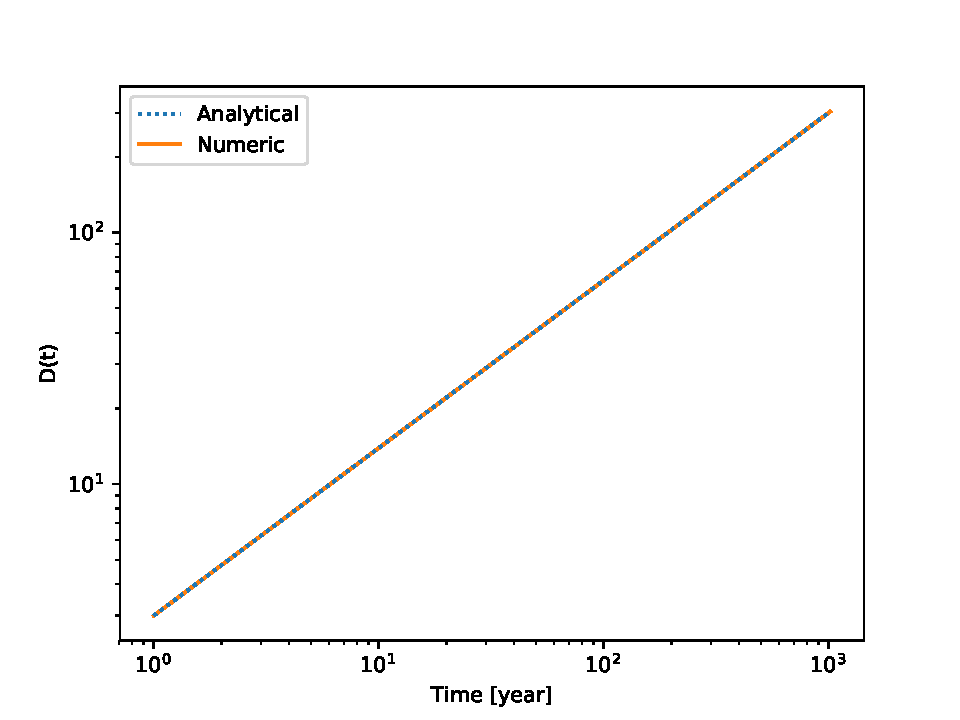
\includegraphics[width=14cm, height=8.5cm]{./Plots/3_ode_0.pdf}
\caption{The analytical (blue) and numerical (orange) solution of the ODE with initial conditions $D(1) = 3, D'(1) = -10$. The plots show that he numerical solution does not appear to have a visible deviation from the analytical solution for the given time interval.}
\end{figure}

\begin{figure}[!ht]
\centering
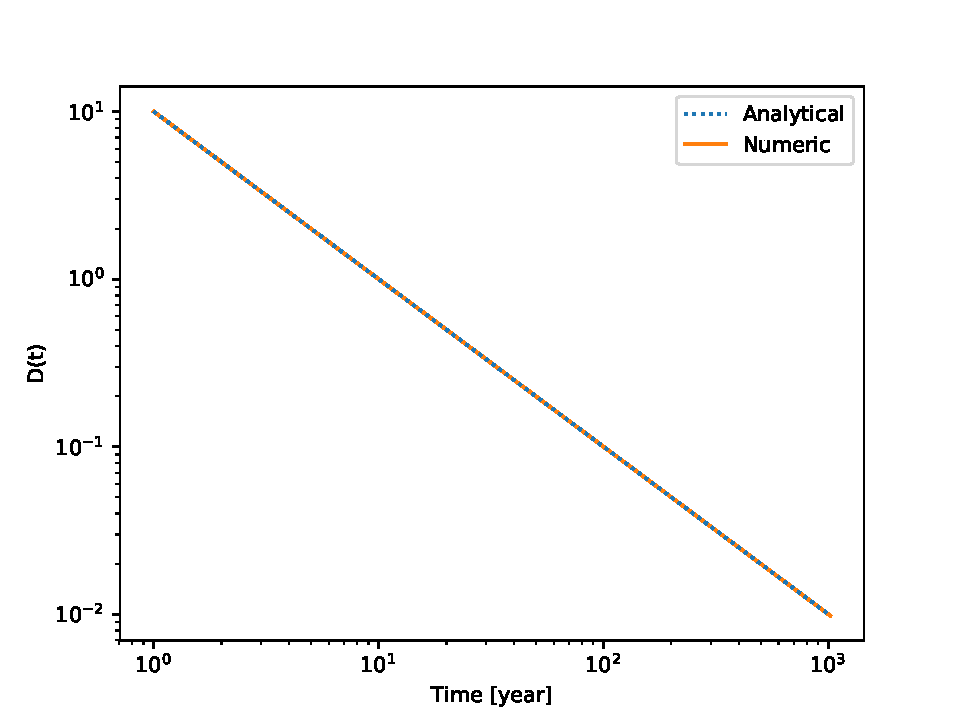
\includegraphics[width=14cm, height=8.5cm]{./Plots/3_ode_1.pdf}
\caption{The analytical (blue) and numerical solution (orange) of the ODE with initial conditions $D(1) = 10,  D'(1) = -10$. The plots show that he numerical solution does not appear to have a visible deviation from the analytical solution for the given time interval.}
\end{figure}
\newpage


\begin{figure}[!ht]
\centering
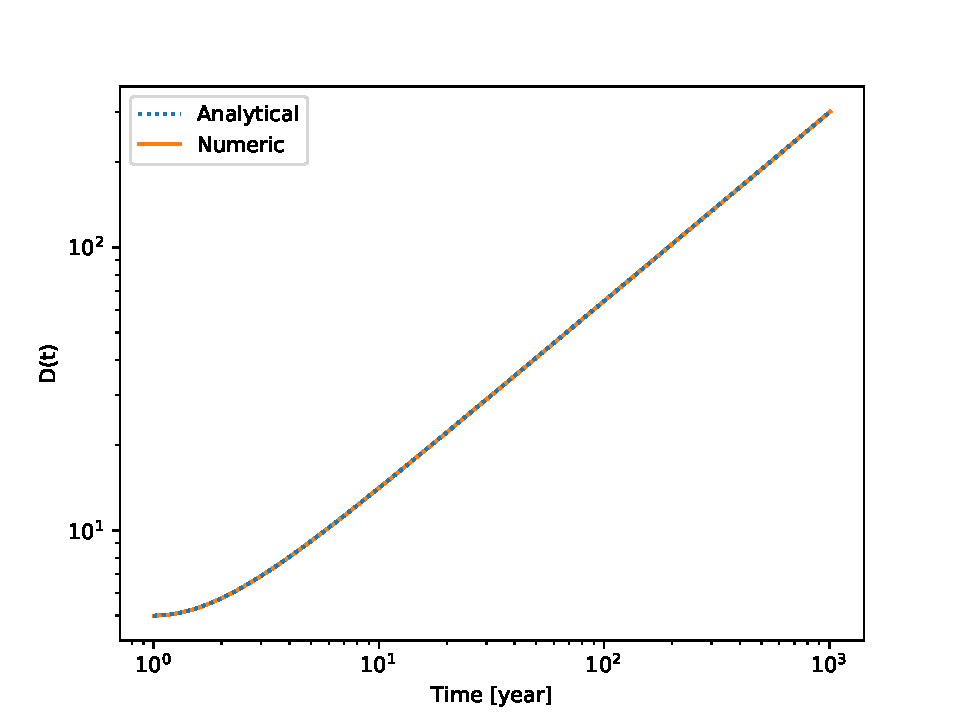
\includegraphics[width=14cm, height=8.5cm]{./Plots/3_ode_2.pdf}
\caption{The analytical (blue) and numerical (orange) solution of the ODE with initial conditions $D(1) = 5,  D'(1) = 0$. The plots show that he numerical solution does not appear to have a visible deviation from the analytical solution for the given time interval.}
\end{figure}

\end{quote}
\end{quote}







\section*{\textbf{4 - Zeldovich approximation} \hrule} 



\subsection*{\textbf{Question 4.a)}}
\begin{quote}

\textbf{Problem}
\begin{quote} 
The linear growth factor is expressed in terms of a integral expression given by,

\begin{equation}
D(z) = \frac{5 \Omega_m H_0^2}{2}H(z) \int_{z}^{\infty} \frac{1+z'}{H^3(z')}dz'
\label{eq:lg}
\end{equation}

Here $z$ is the redshift, $\Omega_m$ is the matter fraction of the Universe at $z = 0$ ($\Omega_m = 0.3$), $H_0$ is the Hubble constant at $z = 0$ and $H(z)$ is the redshift dependent Hubble parameter given by,

\begin{equation}
H(z)^2 = H_0^2 \left(\Omega_m(1+z)^3 + \Omega_{\Lambda} \right)
\end{equation}

Here $\Omega_{\Lambda}$ is the dark energy fraction of the Universe given by $\Omega_{\Lambda} = 0 .7.$ Use numerical integration to calculate the growth factor at $z = 50$ with a relative accuracy of $10^{-5}$. Note that $D(a(z=50))=D(z=50)$, so use either variable.

\end{quote}

\textbf{Solution} 
\begin{quote}
The equation is before integrating first written in terms of the scale factor $a$. Substituting $a = 1/(1+z)$ yields,
\begin{equation}
dz = -(1+z)^2 da = -a^{-2} da
\end{equation}
Plugin this in by equation \ref{eq:lg} results in,

\begin{equation}
D(a) = \frac{5 \Omega_m H_0^2}{2}H(a) \int_{a}^{0} \frac{-a'^{-3}}{H^3(a')} da' = \frac{5 \Omega_m H_0^2}{2}H(a) \int_{0}^{a} \frac{a'^{-3}}{H^3(a')} da'
\label{eq:Dd}
\end{equation}

The Hubble parameter in terms of the scale factor $a$ given by,
\begin{equation}
H(a)^2 = H_0^2 ( \Omega_m a^{-3} + \Omega_{\Lambda} )
\end{equation}

Substituting  this in equation \ref{eq:Dd} and simplifying yields,
\begin{align}
D(a) &= \frac{5 \Omega_m H_0^3}{2} ( \Omega_m a^{-3} + \Omega_{\Lambda} )^{0.5} \int_0^{a} \frac{a'^{-3}}{\left(H_0^2( \Omega_m a^{-3} + \Omega_{\Lambda} ) \right)^{3/2}} da' \\
&= \frac{5 \Omega_m}{2}  ( \Omega_m a^{-3} + \Omega_{\Lambda} )^{0.5} \int_0^{a'} \frac{a'^{-3}}{\left(\Omega_m a^{-3} + \Omega_{\lambda}\right)^{3/2}} da'
\label{EQ:Stuffffff}
\end{align}
The above integral is with the help of Romberg integration solved for $\Omega_{m} =0.3$ and $\Omega_{\lambda} = 0.7$.  The code for Romberg integration can be found at page 57.  The code that prints the output and the printed output can be found below. The shared modules used by the code start at page 53. %code does make use of a function that is needed in assignment 4. This function is located in the shared module ... on page ...
\end{quote}

\textbf{Code - Output}
\begin{quote}
The code that prints the value of the linear growth factor.The code for the called helper function, \texttt{helpers4.calculate\_ linear\_ growth} can be found on page 53.
\lstinputlisting[firstline = 36, lastline=54]{./Code/assigment_4.py}
\end{quote}

\textbf{Text - Output} \\

The output produced by the above code.
\begin{quote}
\lstinputlisting[firstline=0,lastline=1]{./Output/assigment4_out.txt}
\end{quote}

\end{quote}






\newpage
\subsection*{\textbf{Question 4.b)}}
\begin{quote}

\textbf{Problem}
\begin{quote} 
Use your result from the previous question to analytically calculate for $a = 1/51$,
\begin{equation}
\dot{D(t)} = \frac{dD(a)}{da}\dot{da}
\label{EQ:weird}
\end{equation}

Bonus points if you calculate it numerically and match the analytical result within $10^{-8}$. 
\end{quote}

\textbf{Solution} 
\begin{quote}
In this question the derivative is not only calculated analytically, but also numerically. The numerical calculation is performed with ridders method. The analytical solution is derived below and evaluated. The code for the numerical solution and the code that prints the analytical solution\footnote{The analytical solution is printed to make it easier to compare.} can be found after this derivation. This includes the code for ridders method.
\\

To simplify the derivation we define,
\begin{equation}
C = \int_{0}^{a'} \frac{a'^{-3}}{\left( \Omega_m a'^{-3} + \Omega_{\Lambda} \right)^{3/2}} da'
\end{equation}

The derivative can then by substituting 33 in equation 34 be written as,

\begin{align}
\dot{D}(t) &= \frac{5 \Omega_m}{2} \left( \frac{-3 \Omega_m a^{-4}}{2} \left(\Omega_m a^{-3} + \Omega_{\Lambda} \right)^{-0.5}C + \left(\Omega_m a^{-3} + \Omega_{\Lambda} \right)^{0.5} \frac{a^{-3}}{\left( \Omega_m a^{-3} + \Omega_{\Lambda} \right)^{3/2} }  \right) \dot{a} \\
&= \frac{5 \Omega_m}{2} \left( \frac{-3 \Omega_m a^{-4}}{2 \left(\Omega_m a^{-3} + \Omega_{\Lambda} \right)^{0.5}}C + \frac{a^{-3}}{\left( \Omega_m a^{-3} + \Omega_{\Lambda} \right)} \right) \dot{a}
\end{align}

Substituting $\dot{a} = H(a)a(t) = H_0 \left(\Omega_m a^{-3}  + \Omega_{\Lambda} \right)^{0.5}a(t)$ results in,

\begin{align}
\dot{D} &= \frac{5 \Omega_m H_0}{2} \left( \frac{-3 \Omega_m a^{-3}}{2}C + \frac{a^{-2}}{\left( \Omega_m a^{-3} + \Omega_{\Lambda} \right)^{0.5}}  \right)  \\
&= \frac{5 \Omega_m H_0}{2 a^2} \left( \frac{1}{\left(\Omega_m a^{-3} + \Omega_{\Lambda} \right)^{0.5}} - \frac{3\Omega_m}{2a} C \right)
\end{align}

The above expression is evaluated in the code. The value of $C$ is numerically calculated for the analytical expression. This value is just the result of the previous question without scale factor and was allowed to be used for this question. The analytical output (with the numerical calculation for C) and the numerical output (with ridders method) can be found after the code section.

\end{quote}
\newpage

\textbf{Code - Print} \\

\begin{quote}
The code that prints the analytical and numerical result. The code for ridders method follows after
this.
\lstinputlisting[firstline = 55, lastline=96]{./Code/assigment_4.py}
\end{quote}

\textbf{Code - Ridder} \\

\begin{quote}
The code for ridders method.
\lstinputlisting{./Code/mathlib/derivative.py}
\end{quote}

\textbf{Text - Output} \\

The analytical and numerical result. As can be seen is the numerical approximation within $10^{-8}$. 
\begin{quote}
\lstinputlisting[firstline=2,lastline=3]{./Output/assigment4_out.txt}
\end{quote}
\end{quote}







\subsection*{\textbf{Question 4.c)}}
\begin{quote}

\textbf{Problem}
\begin{quote} 
Use the Zeldovich approximation to generate a movie of the evolution of a volume in two dimensions
from a scale factor of 0.0025 until a scale factor of 1.0. To do this, start with 64x64 particles arranged in a square grid with a grid spacing of 1 Mpc. Use $P(k) = k^{-2}$ and the given equation to generate $c_k$, then use the FFT on your grid of particles to calculate $\textbf{S(q)}$. As $a$ increases, update the positions and momenta of the particles and save each step as a frame for your movie. 
\end{quote}

\textbf{Solution} 
\begin{quote}
The difficulty of this exercise lays by the calculation the components of the displacement vector. A brief description of how this is done can be found below.
\\

The displacement vector is calculated by first creating a matrix in $k$ -space with complex values based on the given power law (similar to exercise 2). The matrix is next given the correct hermitian symmetry (see again exercise 2). The components of the displacement vector, $s_x$ and $s_y$, are then calculated independent with the help of this matrix.  This calculation is done as follows. The hemitian matrix is copied and the components in the matrices are multiplied with the wavenumbers and the complex number $i$. The wavenumbers by which the components are multiplied depends on whether we want $s_x$ or $s_y$. The result is two matrices where the cells have respectively values of $ic_k k_x$ and $ic_k k_y$. After this multiplication the matrices cannot be directly fourier transformed to obtain $s_x$ and $s_y$, as the multiplication with the wavenumbers breaks the symmetry in the columns with nyquest wavenumbers. The symmetry is only broken by a minus sign and this is corrected before doing the IFFT. 
\\
The code that creates the movie and the plots for the first 10 particles can be found below. The final plot of the movie is also included and shows that the particles clearly move to the denser region (see figure 25 on page 47).

\end{quote}
\newpage


\textbf{Code - Plots}:
\begin{quote}

The code that creates the movie and the plots of the first 10 particles. The code does make use of an object called 'random' and a function called \texttt{gen\_ complex}. This object and the function  can be found on page 53. The code for the imported shared modules can also be found at page 53. The movie can be found in the movie folder.
\lstinputlisting[firstline = 98, lastline=227]{./Code/assigment_4.py}
\end{quote}

\newpage

\textbf{Plots - Field}

\begin{quote}
\begin{figure}[!ht]
\centering
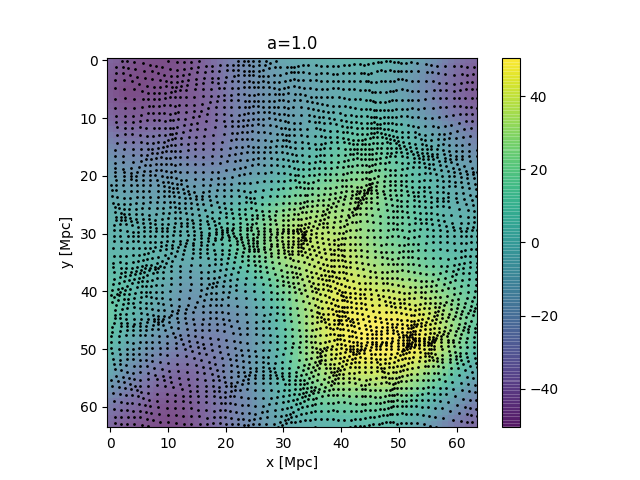
\includegraphics[width=14cm, height=9.5cm]{./Plots/4c/4c=89.png}
\caption{The final plot of the movie. It can clearly be seen that the particles (black dots) moved to the denser region. }
\label{FIG:stuff}
\end{figure}
\end{quote}

\textbf{Plots - particles}
\begin{quote}
\begin{figure}[!ht]
\centering
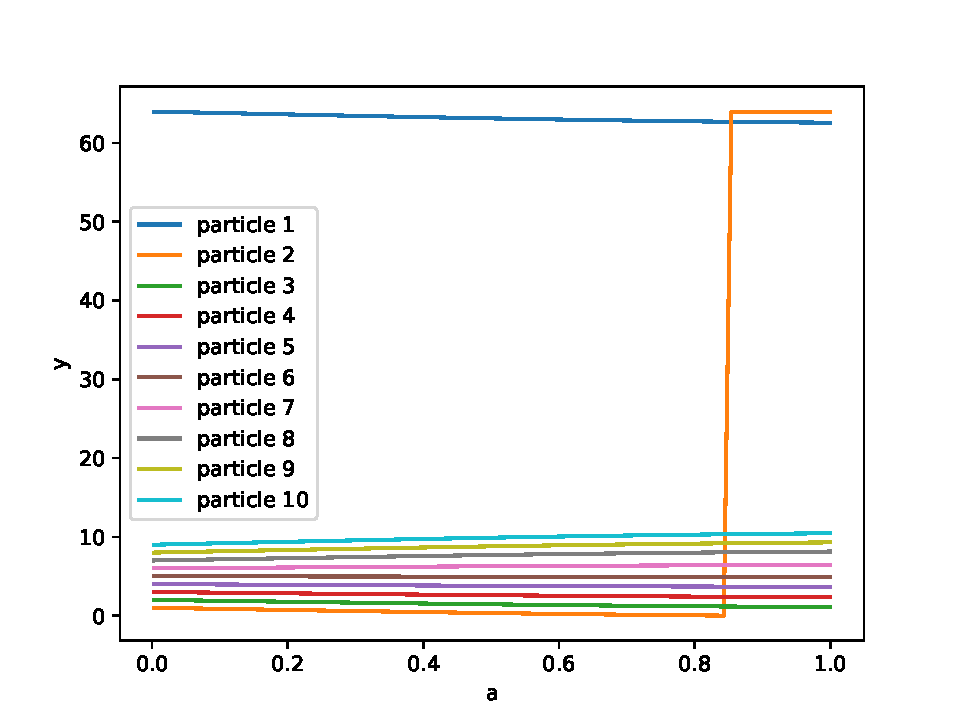
\includegraphics[width=14cm, height=8.5cm]{./Plots/4c_pos.pdf}
\caption{The y-positions of the first 10 particles as function of the scale factor. The plot shows that the particles are slowly moving to a denser region (see figure 25, where the first 10 particles are at the left top). The large jump for particle 2 (orange) at a scale factor of around $ a \approx 0.8$ is the result of the circular boundary conditions.  }
\end{figure}

\begin{figure}[!ht]
\centering
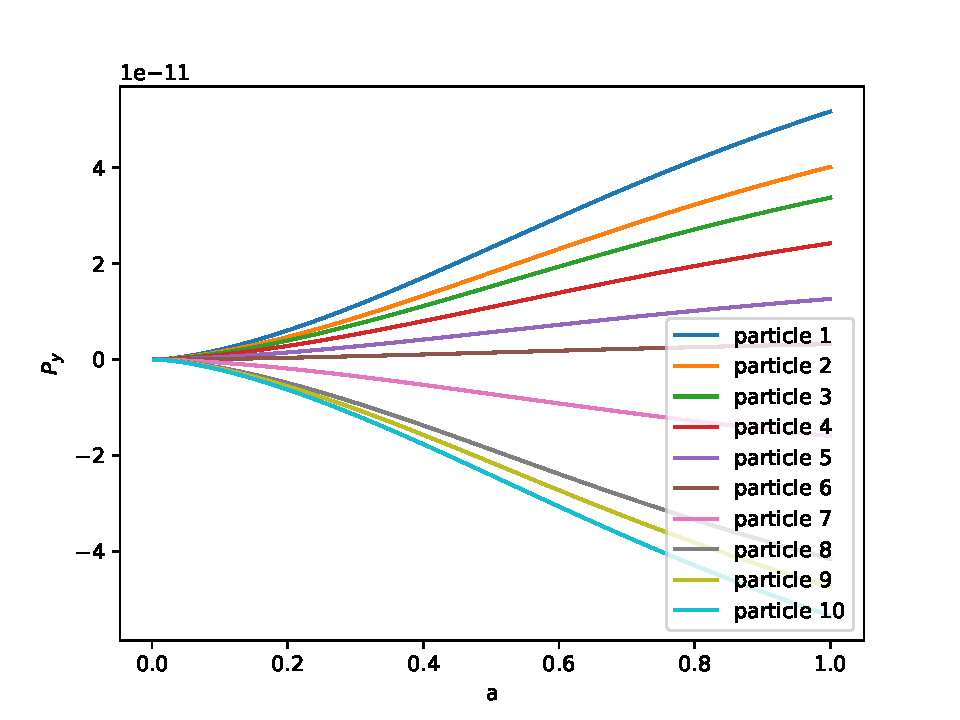
\includegraphics[width=14cm, height=8.5cm]{./Plots/4c_momentum.pdf}
\caption{The momentum of the first 10 particles as function of the scale factor. The fact that about halve of the particles have a positive momentum and that the other halve have a negative momentum is the result of the circular boundary conditions and the created field.  }
\end{figure}
\end{quote}
\end{quote}






\subsection*{\textbf{Question 4.d}}
\begin{quote}

\textbf{Problem}
\begin{quote} 
Generate initial conditions for a three dimensional box to do a N-body simulation, make initial conditions for $64^3$ particles starting at redshift $z = 50$. Besides this make 3 sperate movies of a slice of thickness 1/64th of your box at its center, make a slice for $x-y$, $x-z$,$y-z$. Again make a movie of at least 3 seconds with at least 30 frames per second. Finally plot the position and momentum of the first 10 particles along the $z-direction$ vs $a$.
\end{quote}

\textbf{Solution} 
\begin{quote}
The method in which the displacement vector is similar to the method in 4c. This thus means that first a 3D matrix (tensor) is created in k-space with complex values based on the given power law. The matrix is next given the correct hermitian symmetry, which is done by an extended version of the algorithm explained in question 2. The symmetric matrix (tensor) is now used to calculate the components $s_x$, $s_y$ and $s_z$. This is  done by multiplying the terms in the tensor with the correct wavenumbers and $i$. In the end this results in three matrices that need to be inverse fourier transformed to obtain the components of $\textbf{S}$. The three matrices can however not directly be inverse fourier transformed as the multiplication with the wavenumbers breaks the symmetry in the nyquest planes. The symmetry is again only broken by a minus sign and is first corrected before doing the IFFT. The corrected matrices are then used to calculate $s_x$, $s_y$ and $s_z$. 
\\
The code that uses the displacement vector to creates the simulation and the plots for the first 10 particles can found below.

\end{quote}

\textbf{Code -plots}:
\begin{quote}

The code that creates the movie and the plots of the first 10 particles. 
\lstinputlisting[firstline = 27, lastline=158]{./Code/assigment_4.py}
\end{quote}


\textbf{Plots - particles}
\begin{quote}
\begin{figure}[!ht]
\centering
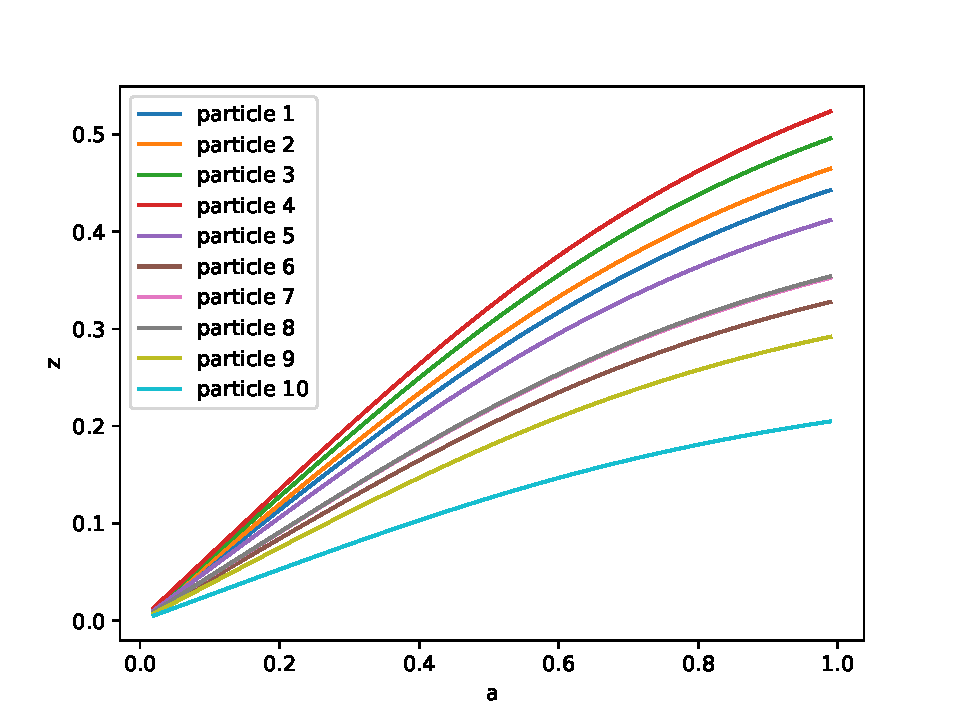
\includegraphics[width=14cm, height=9.5cm]{./Plots/4d_pos.pdf}
\caption{The z-positions of the first 10 particles against the scale factor.}
\end{figure}
\newpage
\begin{figure}[!ht]
\centering
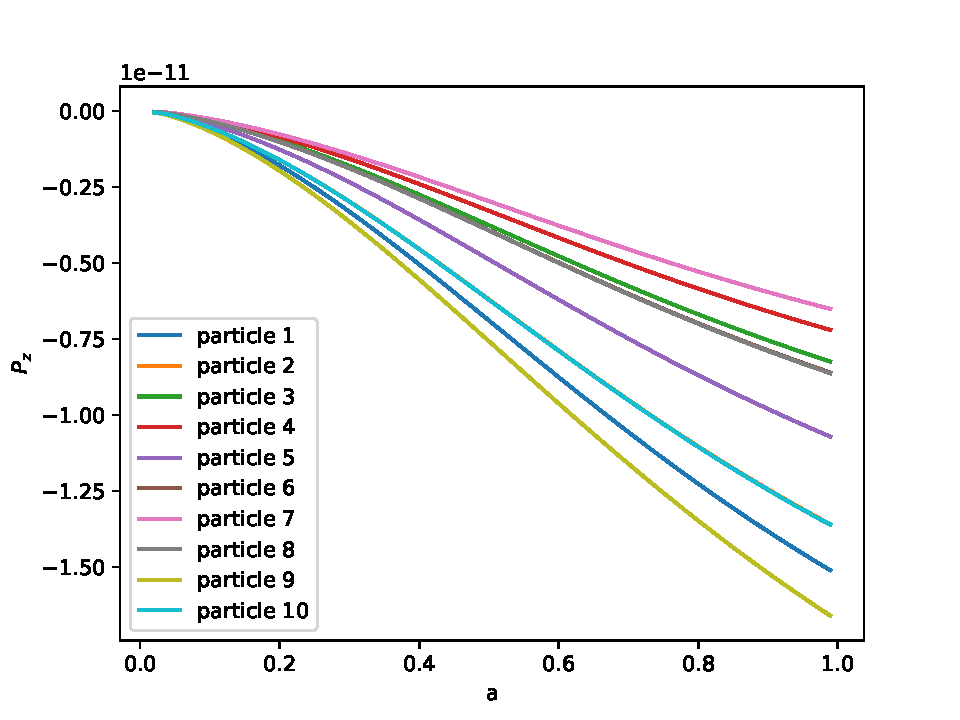
\includegraphics[width=14cm, height=9.5cm]{./Plots/4d_momentum.pdf}
\caption{The z-component of the momentum of the first 10 particles against the scale factor. }
\end{figure}
\end{quote}



\end{quote}






\subsection*{\textbf{Question 4- Summary}}
\begin{quote}

\textbf{Summary}
\begin{quote}
The current sub-section contains the summary of the code used for assignment 4. This includes the part of the main file that executes the subquestions and the relevant imports, the functions to calculate the linear growth factor and the functions used to generate and sort the matrices.

\end{quote}


\textbf{Code - Assignment}

\begin{quote}
The code with the main function and the function \texttt{gen\_complex}, which is called in 4c and 4d. 
\label{CODE:MAIN4}
\lstinputlisting[firstline=0,lastline=32]{./Code/assigment_4.py}
\end{quote}

\newpage
\textbf{Code - Shared-modules} \\
\begin{quote}
\textbf{Linear growth} \\
The code which calculates the linear growth factor and the derivative of the liner growth factor.
\label{CODE:h4}
\lstinputlisting{./Code/mathlib/helpers4.py}
\end{quote}

\begin{quote}
\textbf{Tensor/matrix} \\
The code containing all the function sued to create the matrices (tensors) and make then symmetric.  
\lstinputlisting{./Code/mathlib/misc.py}
\label{CODE:misc}
\end{quote}
\end{quote}

\newpage

%\textbf{Code - output } 
%\begin{quote}
% The code that produces the output.
%\lstinputlisting{./code/assigment1_a.py}
%\end{quote}

%\textbf{Code - helper } 
%\begin{quote}
%The code for the Poisson distribution and the factorial function.  
%\lstinputlisting[firstline=2,lastline=46]{./code/mathlib/utils.py}
%\end{quote}


%\textbf{Output}
%\begin{quote}
%The output produced by \textsf{/code/assigment1\_ a.py} 
%\lstinputlisting{./output/assigment1_a_out.txt}
%\end{quote}
\newpage















\section*{\textbf{5 - Mass assignment schemes} \hrule} 



\subsection*{\textbf{Question 5.a}}
\begin{quote}

\textbf{Problem}
\begin{quote}
The most simple choice for the particle shape is a point like shape given by:
\begin{equation}
S(x) = \frac{1}{\Delta x} \delta \left(\frac{x}{\Delta x} \right)
\end{equation}

Explain how we need to assign mass to the grid in this scheme and explain why this method is called the Nearest Grid Point (NGP) method. Code up your own implementation of the mass assignment scheme NGP, using a grid of $16^3$. 
Display x-y slices of the grid with $z$ values of 4,9,11 and 14.
\end{quote}

\textbf{Solution} 
\begin{quote}
The easiest way of assigning the mass of the particles to a grid is by assigning it to the grid points.  For the given particle shape this would correspond to assigning the full mass of a particle to its nearest gird point, from which the name follows. For other particle shapes, such as the cloud in a cell shape, the mass might be fully assignment to the nearest gird point, but it might also be partially assigned to multiple grid points. % (depending on the position of the particle).
\\
The mass is for the given  particle shape assigned to the gird points by abusing the fact that a cast to an integer always result in down a cast (i.e 15.7 casted to an integer gives 15). The indices of a grid point to which a particle has to assign its mass can, by abusing the down cast, be found by adding 0.5 to the position and then down casting the result to an integer.  To include circular boundary conditions the modulo with 16 (grid size) is taken. 

%the particles have to assign their mass can be found by adding 0.5 to the position of a particle and then casting it to an integer. To include circular boundary conditions the modulo with 16 (grid size) is taken of the result. % (i.e 15.6 + 0.5 = 16.1, int cast -> 16 , mod -> 0)

The code that creates the plots with the slices and the plots can be found below. The code that assigns the mass can be found in the shared module \texttt{./Code/mathlib/mass.py} on page 73
\end{quote}

\textbf{Code - slices}
\begin{quote}
The code that creates the plots with the slices of the mass grid.
\lstinputlisting[firstline = 14, lastline=40]{./Code/assigment_5.py}
\end{quote}

\newpage

\textbf{Plots - Slices}
\begin{quote}
\begin{figure}[!ht]
\centering
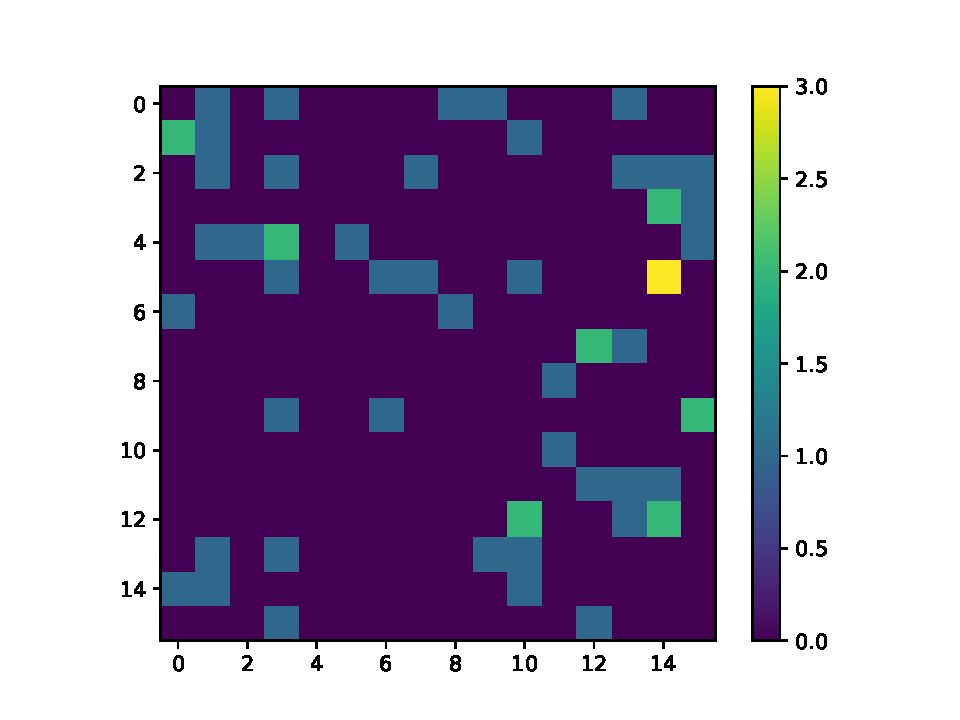
\includegraphics[width=14cm, height=9.5cm]{./Plots/5a_slice_4.pdf}
\caption{The x-y slice of the created mass grid for $z = 4$. The color indicates the assigned mass in terms of particle mass. }
\end{figure}


\begin{figure}[!ht]
\centering
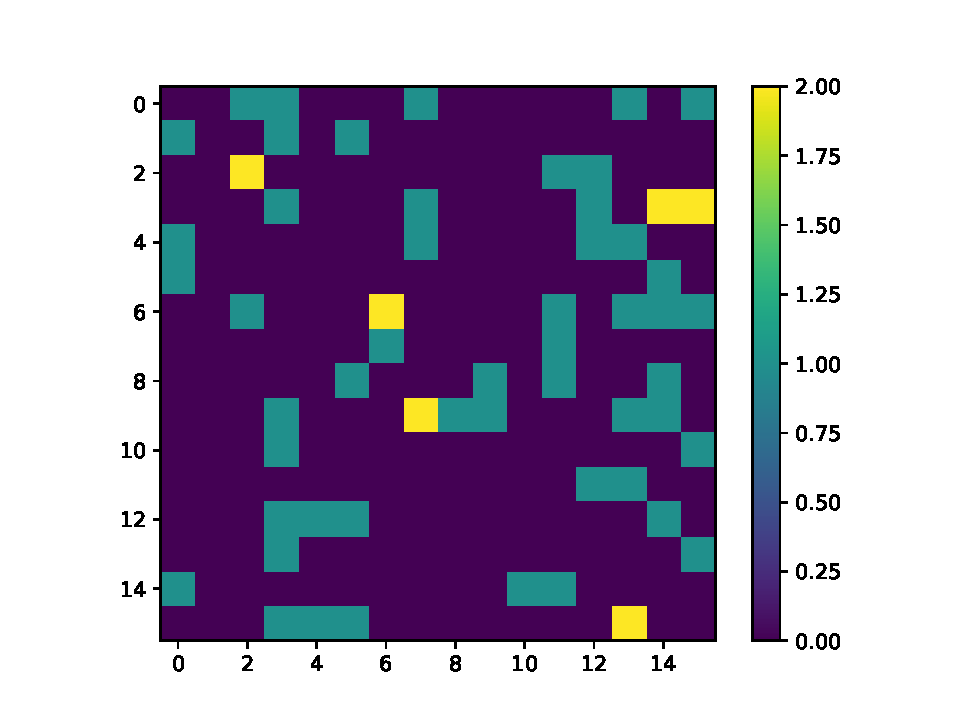
\includegraphics[width=14cm, height=9.5cm]{./Plots/5a_slice_9.pdf}
\caption{The x-y slice of the created mass grid for $z = 9$. The color indicates the assigned mass in terms of particle mass. Notice that the range of the colorbar is different from the first and last plot.}
\end{figure}
\newpage

\begin{figure}[!ht]
\centering
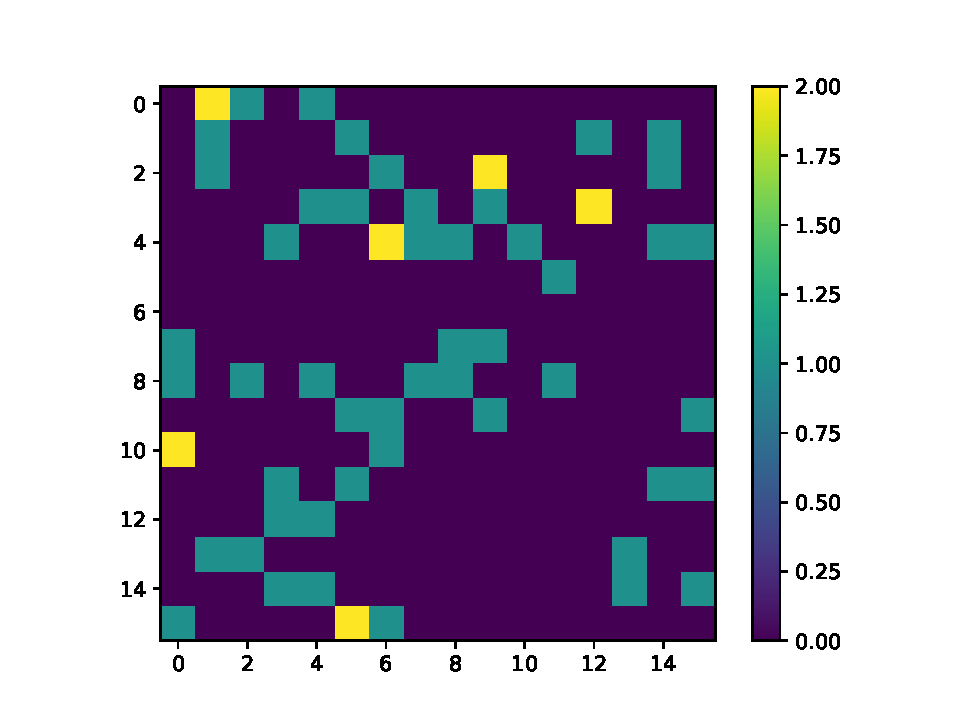
\includegraphics[width=14cm, height=9.5cm]{./Plots/5a_slice_11.pdf}
\caption{The x-y slice of the created mass grid for $z = 11$. The color indicates the assigned mass in terms of particle mass. Notice that the range of the colorbar is different than the first and last plot. }
\end{figure}

\begin{figure}[!ht]
\centering
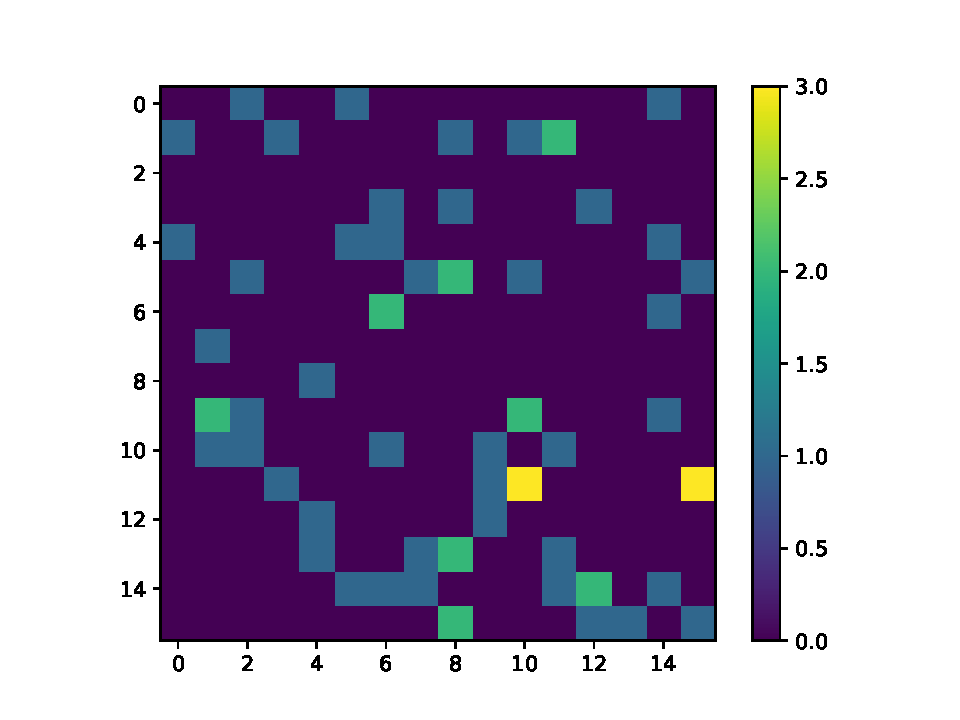
\includegraphics[width=14cm, height=9.5cm]{./Plots/5a_slice_14.pdf}
\caption{The x-y slice of the created mass grid for $z = 14$. The color indicates the assigned mass in terms of particle mass. }
\end{figure}
\end{quote}
\newpage
\end{quote}













\subsection*{\textbf{Question 5.b)}}
\begin{quote}

\textbf{Problem}
\begin{quote}
To check the robustness of your implementation make a plot of the x position of an individual particle and the value in cell 4 in 1 dimension and let x vary from the lowest value to the highest possible value in $x$. Repeat for cell 0.
\end{quote}

\textbf{Solution} 
\begin{quote}
There is not much to explain here, besides that the results for cell 4 and cell 0 are shown in the same plot. The code that creates the plot and the plot can be found below.

\end{quote}

\textbf{Code - Plots}
\begin{quote}
The code that creates the plots for cell 0 and cell 4. 
\lstinputlisting[firstline = 41, lastline=72]{./Code/assigment_5.py}
\end{quote}
\newpage

\textbf{Plots - Cell}
\begin{quote}
\begin{figure}[!ht]
\centering
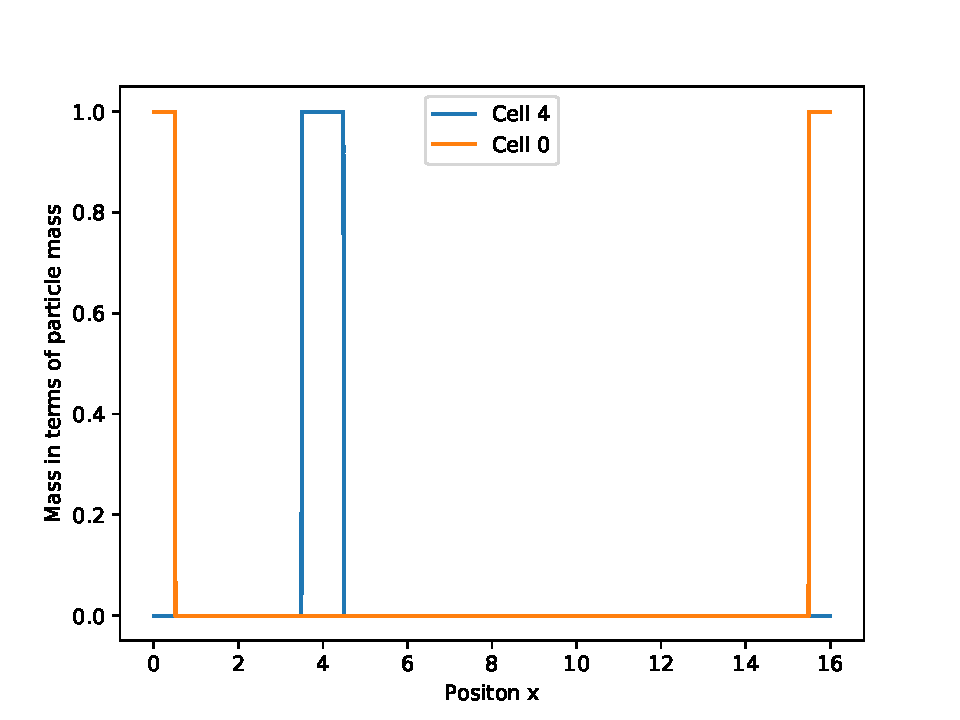
\includegraphics[width=14cm, height=8.5cm]{./Plots/5b_cell.pdf}
\caption{The mass assigned for a particle moving from x = 0 to x = 16. The orange and red line respectively indicate the mass assigned to cells 0 and 4 as function of the position of the particle. The plot is created for a mass grid of size 16 with circular boundary conditions.  }
\end{figure}

\end{quote}
\end{quote}













\subsection*{\textbf{Question 5.c}}
\begin{quote}

\textbf{Problem}
\begin{quote}
Right noew we want to improve this method, because NGP has several disadvantages. For this we are going to use a method which assumes that particles are cubes in 3D of uniform density and have the size of a grid cell. Calculatue how mass needs to be assigned in the case of this other method called the Cloud In Cell (CIC) methoed and implement it in code. To check the robustness of your implementation again make the same plots as before.
\end{quote}

\textbf{Solution} 
\begin{quote}
The mass needs to be assigned over the nearest 8 grid points. Each grid point gets thereby a fraction of the cube around the particle. The fraction assigned to a grid point here depends on the position of the particle and might be zero for some of the nearest 8 grid points. The way in which the mass is assigned to the nearest gird points is explained in the comment of the code that assigns the mass(page ... ). The code that creates the plots and the plots them self can be found below.
\newpage
\end{quote}

\textbf{Code - slices}
\begin{quote}
The code that creates the slices, cell 0 and cell 4 in a 3D grid of size 16.
\lstinputlisting[firstline = 60, lastline=102]{./Code/assigment_5.py}
\end{quote}

\newpage


\textbf{Plots - Slices}
\begin{quote}
\begin{figure}[!ht]
\centering
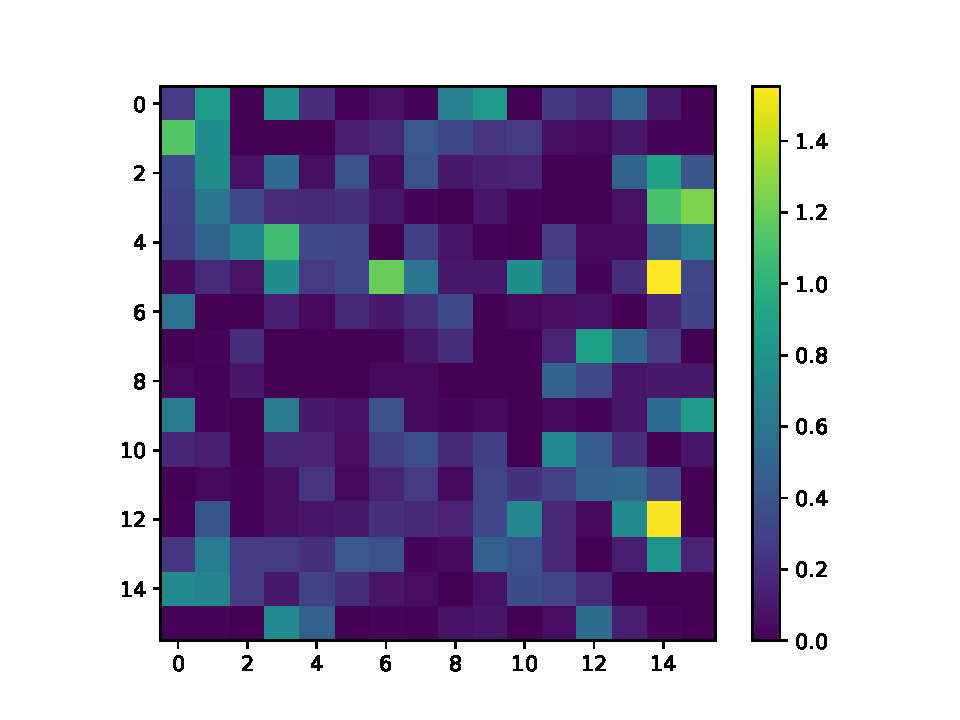
\includegraphics[width=14cm, height=9.5cm]{./Plots/5c_slice_4.pdf}
\caption{The x-y slice of the created mass grid with the CIC method for $z = 4$. The color indicates the assignment mass in terms of particle mass. }
\end{figure}

\begin{figure}[!ht]
\centering
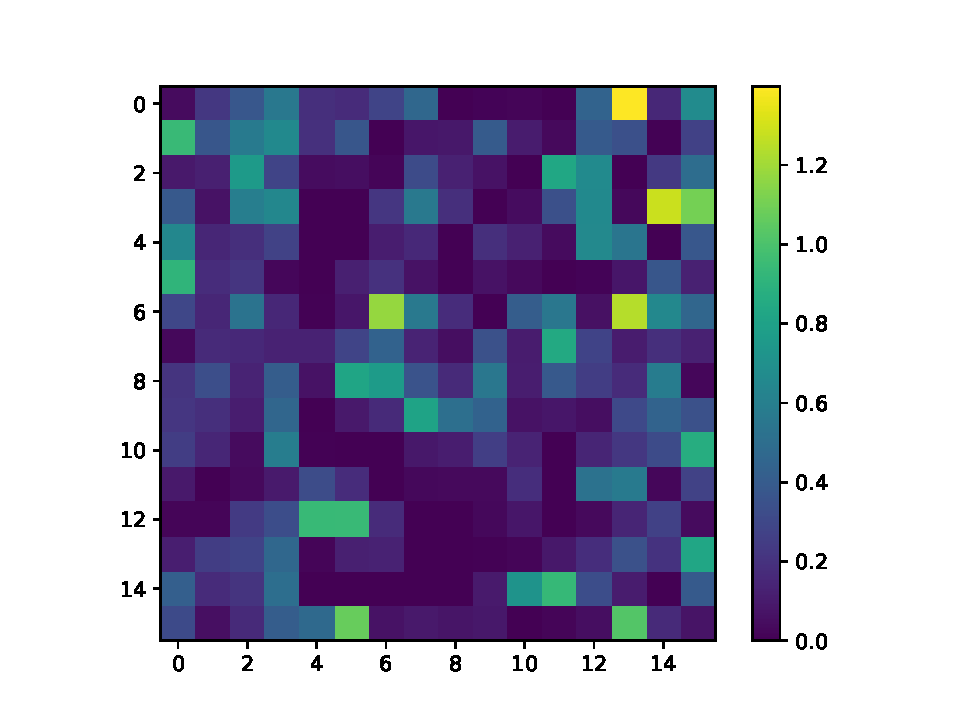
\includegraphics[width=14cm, height=9.5cm]{./Plots/5c_slice_9.pdf}
\caption{The x-y slice of the created mass grid with the CIC method for $z = 9$. The color indicates the assignment mass in terms of particle mass. }
\end{figure}

\newpage
\begin{figure}[!ht]
\centering
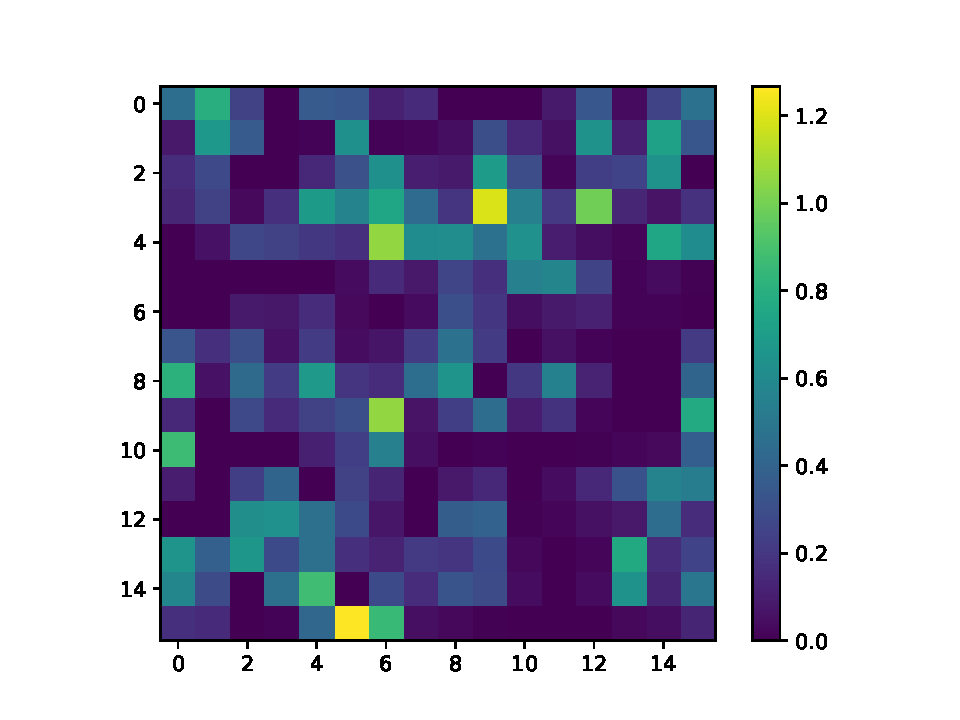
\includegraphics[width=14cm, height=9.5cm]{./Plots/5c_slice_11.pdf}
\caption{The x-y slice of the created mass grid with the CIC method for $z = 11$. The color indicates the assignment mass in terms of particle mass. }
\end{figure}


\begin{figure}[!ht]
\centering
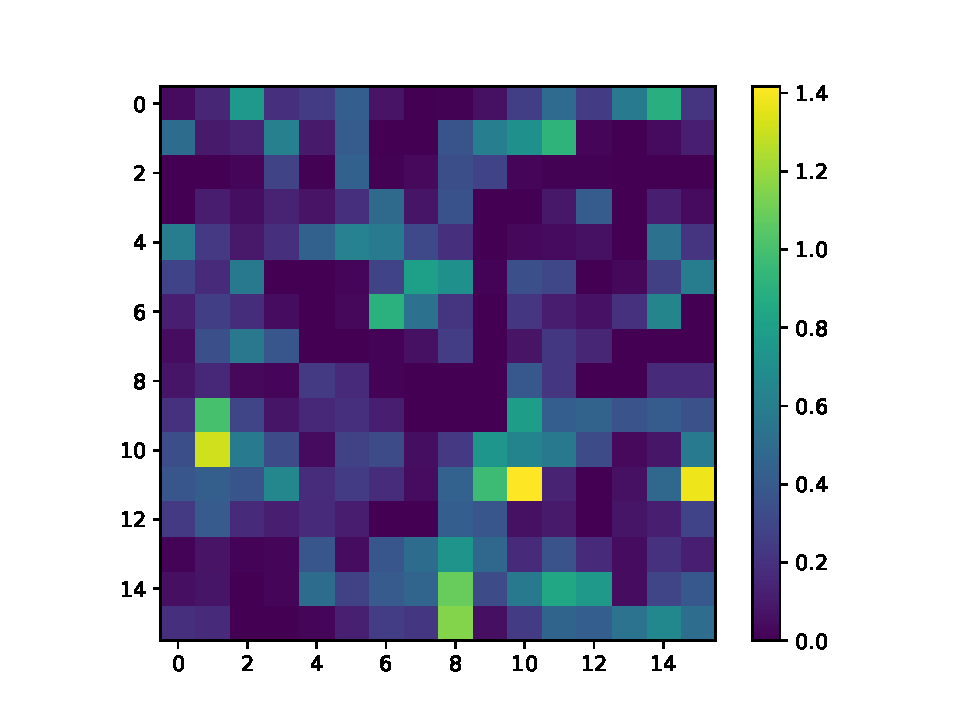
\includegraphics[width=14cm, height=9.5cm]{./Plots/5c_slice_14.pdf}
\caption{The x-y slice of the created mass grid with the CIC for $z = 14$. The color indicates the assignment mass in terms of particle mass. }
\end{figure}
\newpage

\textbf{Plots - Cells}
\begin{quote}
\begin{figure}[!ht]
\centering
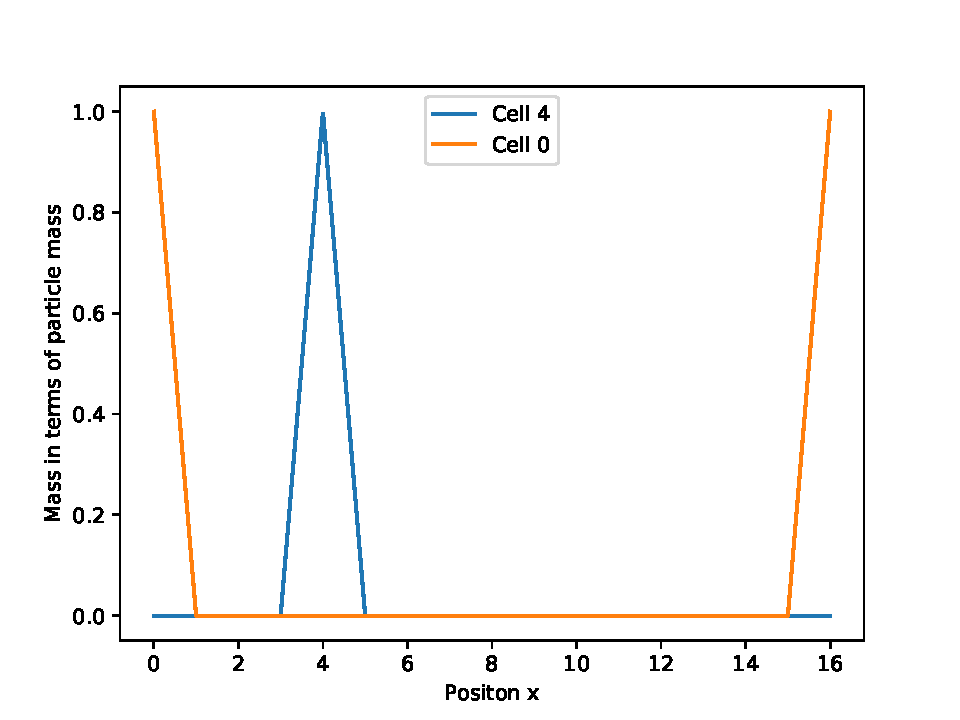
\includegraphics[width=14cm, height=9.5cm]{./Plots/5c_cell.pdf}
\caption{The mass assigned for a particle moving from x = 0 to x = 16 for the cloud in the cell method. The orange and red line respectively indicate the mass assigned to cells 0 and 4 as function of the position of the particle. The plot is created for a 3D  mass grid of size 16 with circular boundary conditions.  }
\end{figure}

\end{quote}
\end{quote}
\end{quote}













\subsection*{\textbf{Question 5.d}}
\begin{quote}

\textbf{Problem}
\begin{quote}
Write your own FFT algorithm; check that your code works with a 1D function (no Gaussian) by making a plot of the FFt and compare your result with a python package and the analytical FFT of your function. In the rest of this exercise you need to use your own FFT. 
\end{quote}

\textbf{Solution} 
\begin{quote}
The created implementation of the FFT consist of an recursive implementation with the Cooley-Tukey algorithm. The implementation doesn't store the data inplace, but in a new array. This choice was made to prevent he input array from being modified. One consequence of this choice is that the input array does not have to be reverse bit shifted. 
\\
The implementation is compared with the numpy implementation. The function that is chosen to fourier transform is the cosine\footnote{The given expression contains a proportional sign as the pre-factor depends on the definition of the Fourier transformation.},

\begin{equation}
\mathcal{F}(\cos(2 \pi At) ]\propto 0.5(\delta(f - A) + \delta(f + A))
\end{equation}
\\
The code for the FFT can be found on page .. in the file .... The code that compares the self written implementation with the numpy implementation and the analytical solution can be found below.  
\newpage

%
%\newpage
%\end{quote}

\textbf{Code - slices}
\begin{quote}
The code that creates the plots for the comparison of the self written FFT with the numpy implementation and the analytical solution.
%The code that creates the slices, cell 0 and cell 4 in a 3D grid of size 16.
\lstinputlisting[firstline = 108, lastline=137]{./Code/assigment_5.py}
\end{quote}

\newpage
\textbf{Plot - Comparison}
\begin{quote}

\begin{figure}[!ht]
\centering
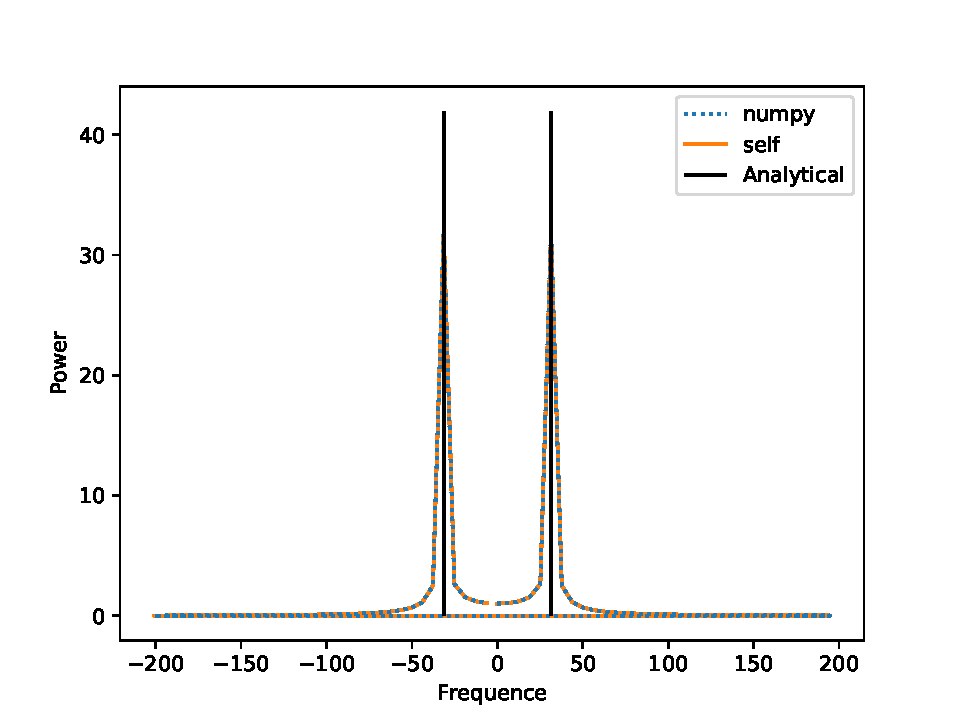
\includegraphics[width=14cm, height=8.5cm]{./Plots/5d_fourier.pdf}
\caption{The own implementation of the FFT (orange), the numpy implementation (blue) and the analytical fft (black). The plot shows that there is now visible deviation from the numpy version. It can also be seen that both the numpy and the self written implementation do not correctly represent the peak of the delta function. This is expected as it would require an infinite amount of samples to obtain the exact same result. }
\end{figure}
\end{quote}
%\newpage


\end{quote}
\end{quote}













\subsection*{\textbf{Question 5.e)}}
\begin{quote}

\textbf{Problem}
\begin{quote}
Generalize your own FFT algorithm to 2 and 3 dimensions and make a plot of the FFT of a 2D function (no bivariate Gaussian) and compare it with the analytical FFT of your FFT. Also make a plot of the FFT of a 3D multivariate Gaussian function, plot 3 slices centered at the center for the 3 different slice options x-y, x-z,y-z.
\end{quote}

\textbf{Solution} 
\begin{quote}

The code for the 2D and 3D implementation makes use of the code for the 1D implementation. In 2D the FFT is first taken over the first axis of the input matrix and then over the second axis. In 3D the FFT2 is first taken over the first axis and then the FFT is taken over the third axis. 
The code is not generalized to N-dimensions, as the question did not ask to write your own swapaxis algorithm. 
\\
The chosen function to 2D fourier transform is $\cos(x+y)$. The analytical result consists of two 2D delta functions. The code that makes the plots for the 2D FFT and the 3D FFT can be found below, the implementation its self can be found on page 75. The plots can be found below the code.
\end{quote}
\newpage

\textbf{Code - Plot}
\begin{quote}
The code that creates the plots.
%The code that creates the slices, cell 0 and cell 4 in a 3D grid of size 16.
\lstinputlisting[firstline = 162, lastline=231]{./Code/assigment_5.py}
\end{quote}

\textbf{Plot - 2D}\\
\begin{quote}

\begin{figure}[!ht]
\centering
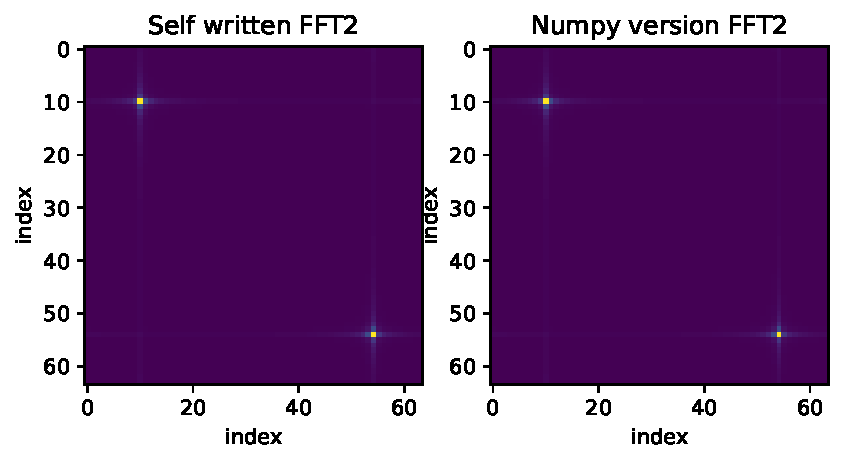
\includegraphics[width=15cm, height=7.5cm]{./Plots/5e_2d_fft.pdf}

\caption{The 2D fourier transformation for the function $\cos(x+y)$. Left, the own implementation of the FFT2 (left) and right the numpy implementation. The results show that the self written version appears to be equal to the numpy version. For the cosine two delta peaks are expected to arise which can also be seen. The peaks are not infinite sharp as that would require an infinite amount of samples. }
\end{figure}
\end{quote}
\textbf{Plot - 3D}
\begin{quote}
\vspace*{-0.5cm}

\begin{figure}[!hb]
\centering
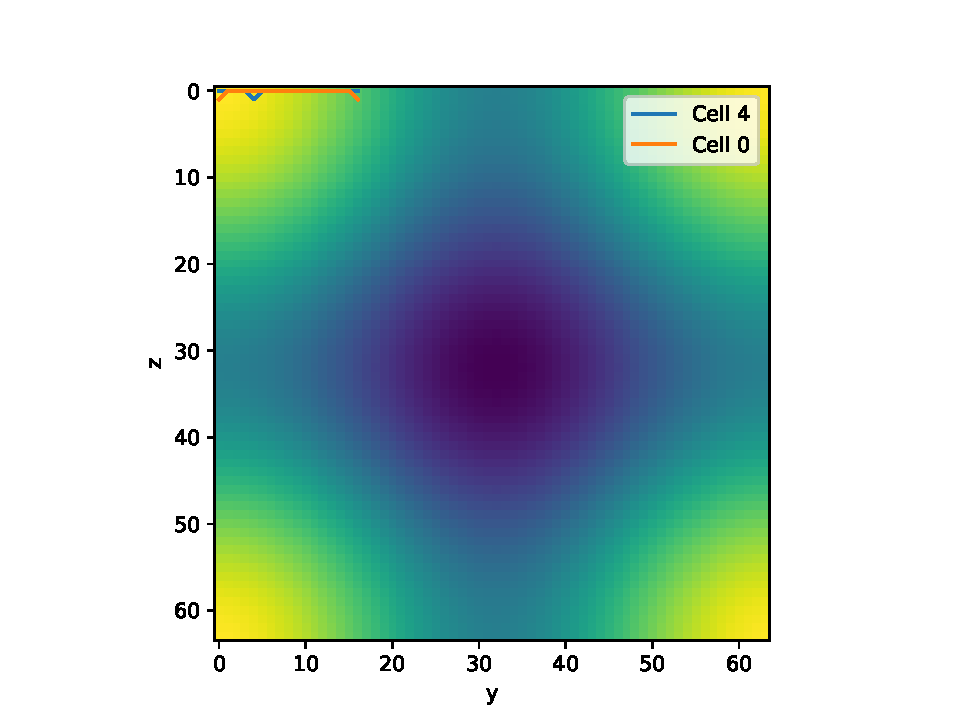
\includegraphics[width=14cm, height=7.5cm]{./Plots/5e_gaussian_yz.pdf}
\caption{The yz slice around the center of the 3D Fourier transform of a multivariate gaussian with $\mu = 0$ and $\sigma = 0.5$.  The slice should be perfectly symmetric and the result shows that this is indeed the case. }
\end{figure}
\newpage

\begin{figure}[!ht]
\centering
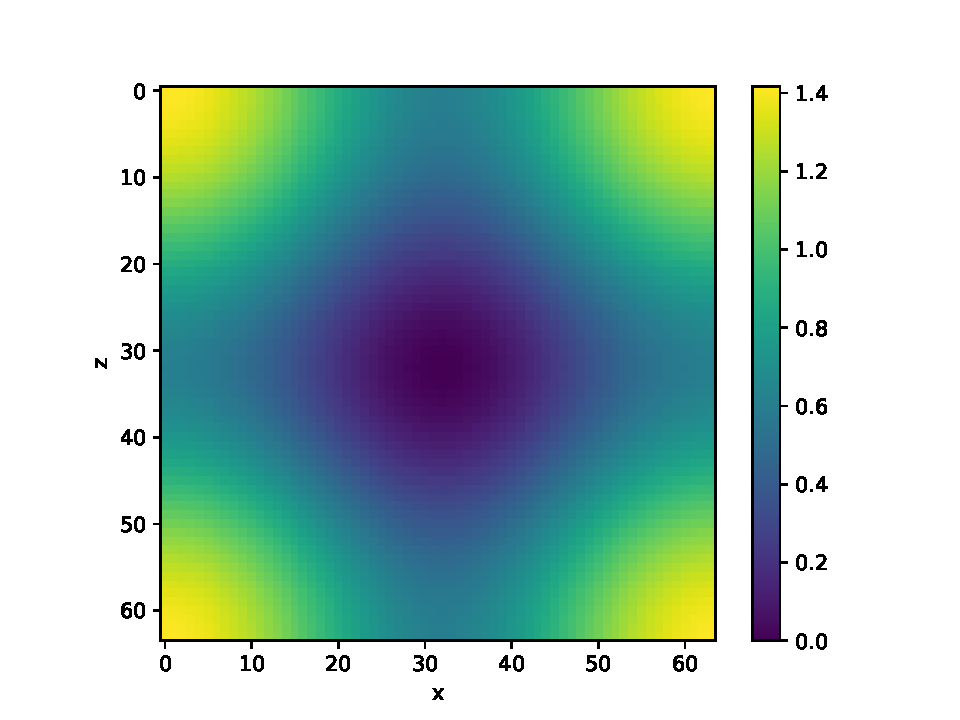
\includegraphics[width=14cm, height=7.5cm]{./Plots/5e_gaussian_xz.pdf}
\caption{The xz slice around the center of the 3D Fourier transform of a multivariate gaussian with $\mu = 0$ and $\sigma = 0.5$.  The slice should be perfectly symmetric and the result shows that this is indeed the case. }
\end{figure}

\begin{figure}[!hb]
\centering
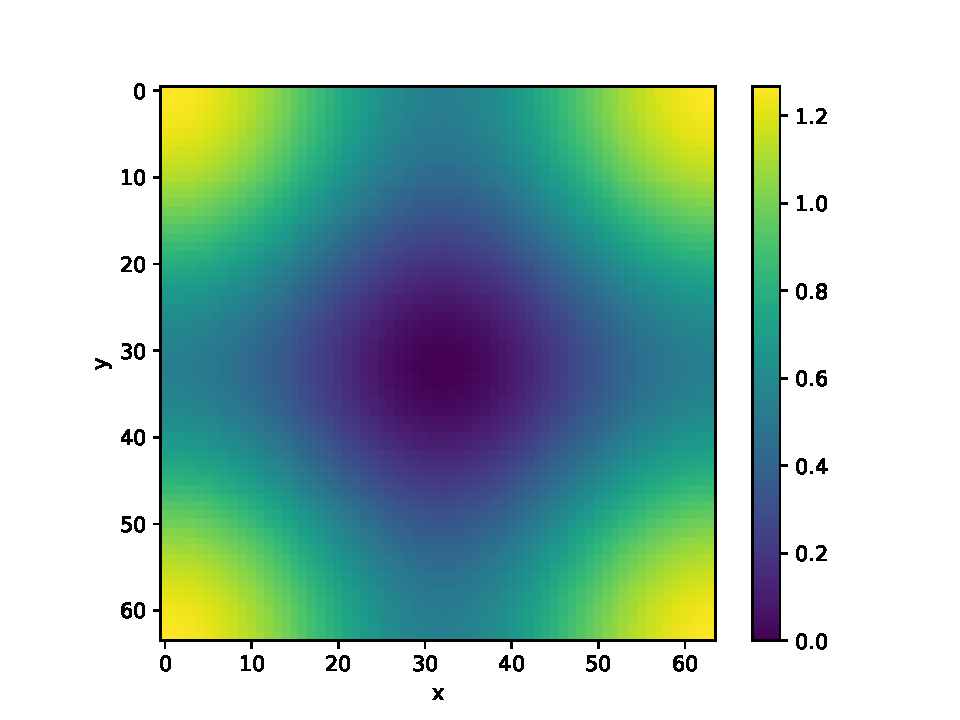
\includegraphics[width=14cm, height=7.5cm]{./Plots/5e_gaussian_xy.pdf}
\caption{The xy slice around the center of the 3D Fourier transform of a multivariate gaussian with $\mu = 0$ and $\sigma = 0.5$.  The slice should be perfectly symmetric and the result shows that this is indeed the case. }
\end{figure}
\end{quote}

\end{quote}

%\end{quote}














\subsection*{\textbf{Question 5 - Summary}}
\begin{quote}

\textbf{Summary}
\begin{quote}
The current sub-section contains the summary of the code used for assignment 5. This includes the part of the main file that executes the subquestions, the relevant imports, the functions to assign the mass for the NGP and CIC method and, the code for the Fourier transformations. %calculate the linear growth factor and the functions used to generate and sort the matrices (tensor).

\end{quote}


\textbf{Code - Assignment}

\begin{quote}
The code with the main function that executes the sub questions and the relevant imports.
\label{CODE:MAIN5}
\lstinputlisting[firstline=0,lastline=12]{./Code/assigment_5.py}
\end{quote}

\textbf{Code - Mass} \\
\begin{quote}
The code that assigns the masses for the NGP and CIC method
\label{CODE:mass}
\lstinputlisting{./Code/mathlib/mass.py}
\end{quote}

\newpage
\textbf{Code - Fourier}
\begin{quote}
The code containing the fourier transformations.   
\lstinputlisting{./Code/mathlib/fourier.py}
\label{CODE:fourier}
\end{quote}


\end{quote}


%\textbf{Code - output } 
%\begin{quote}
% The code that produces the output.
%\lstinputlisting{./code/assigment1_a.py}
%\end{quote}

%\textbf{Code - helper } 
%\begin{quote}
%The code for the Poisson distribution and the factorial function.  
%\lstinputlisting[firstline=2,lastline=46]{./code/mathlib/utils.py}
%\end{quote}


%\textbf{Output}
%\begin{quote}
%The output produced by \textsf{/code/assigment1\_ a.py} 
%\lstinputlisting{./output/assigment1_a_out.txt}
%\end{quote}
\newpage













\section*{\textbf{6 - Classifying x-ray bursts} \hrule} 



\subsection*{\textbf{Question 6}}
\begin{quote}

\textbf{Problem}
\begin{quote}
Use logistic regression to make a model of the data, suing a binary classification for short or long GRBs. Explain which properties your model uses to prediced whether a GRB is short or long, and how you handle missing data. Plot a histogram of the class (0 or 1) of GRB and overplot the actual class based on the value of $T_{90}$.
\end{quote}

\textbf{Solution} 
\begin{quote}


The data is before training the model pre-processed as follows. The first stap consists of removing all rows with missing $T_{90}$ (this only consists of two rows). Next, the columns with  logarithmic values are taken to the power of an exponent. Finally the values of $-1$ in the non logarithmic columns and the values of $e^{-1}$ in the logarithmic columns are replaced with 0. The reason that the columns with logarithmic values where first taken to the exponent is because directly replacing -1.0 in such a column with 0 is equivalent to creating your own data. (i.e if $\ln(M_{*}/M_{\odot}) = 0$, then we would have created data that implies that $M_{*} = M_{\odot}$). 
\\
The columns that where chosen for training  consist of the redshift, the star formation rate and the log of the mass ratio. These columns where selected based on a scatter plot made with seaborn in which all columns where plotted against each other. The code for this is not included\footnote{I did not had enough time to recreate the plot without seaborn before the deadline.}. 
\\
With these columns an accuracy of 78 \% was obtained (see page 80). This value is unfortunately the base line that needs to be broken, as in the final dataset 78\% of all entries are long GRBS. The model is thus returning '1' for each entry. Attempts to use different combinations of columns always resulted in the same accuracy. The code that creates the histogram and the code for the logistic regression can be found below.  

\end{quote}

\textbf{Code - Plot}
\begin{quote}
The code that creates the plots.
%The code that creates the slices, cell 0 and cell 4 in a 3D grid of size 16.
\lstinputlisting{./Code/assigment_6.py}
\end{quote}

\textbf{Code - Logistic regression}
\begin{quote}
The code for logistic regression.
%The code that creates the slices, cell 0 and cell 4 in a 3D grid of size 16.
\lstinputlisting{./Code/mathlib/LogisticRegression.py}
\end{quote}
\newpage

\textbf{Text - Output} \\

The accuracy obtained by the model.
\begin{quote}
\lstinputlisting{./Output/assigment6_out.txt}
\end{quote}

\textbf{Plots- Histogram}
\begin{figure}[!hb]
\centering
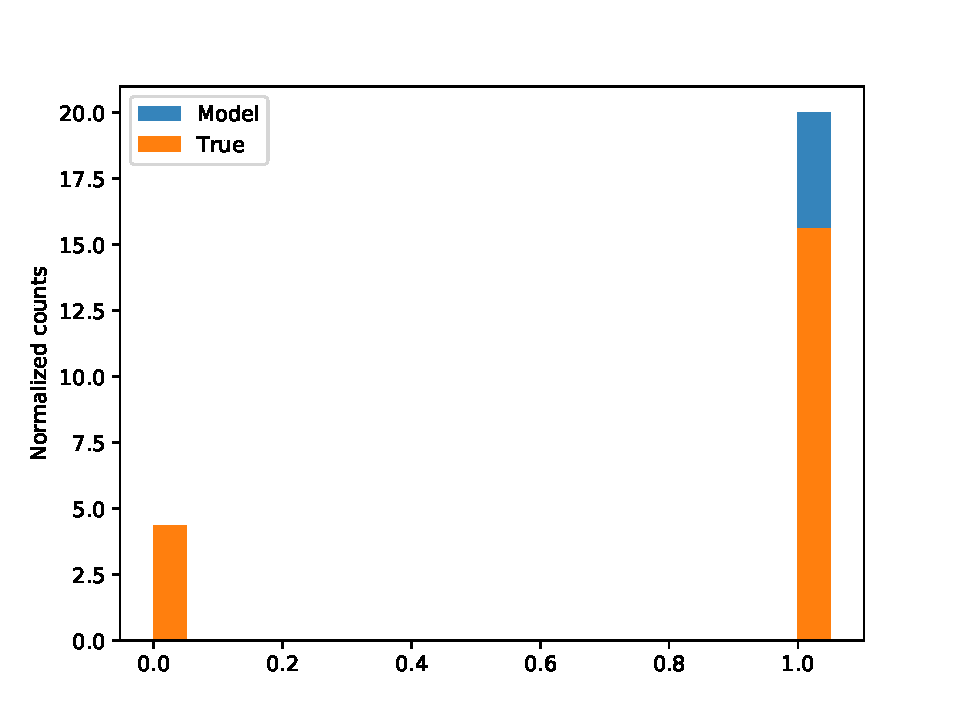
\includegraphics[width=14cm, height=7.5cm]{./Plots/6a_hist.pdf}
\caption{The created histogram for the prediction made by the model and the true labels. It can be seen here that the model always returns '1'. }
\end{figure}

\begin{quote} 


\end{quote}
\end{quote}











%\section*{\textbf{4 - Zeldovich approximation} \hrule} 



\subsection*{\textbf{Question 4.a)}}
\begin{quote}

\textbf{Problem}
\begin{quote} 
The linear growth factor is expressed in terms of a integral expression given by,

\begin{equation}
D(z) = \frac{5 \Omega_m H_0^2}{2}H(z) \int_{z}^{\infty} \frac{1+z'}{H^3(z')}dz'
\label{eq:lg}
\end{equation}

Here $z$ is the redshift, $\Omega_m$ is the matter fraction of the Universe at $z = 0$ ($\Omega_m = 0.3$), $H_0$ is the Hubble constant at $z = 0$ and $H(z)$ is the redshift dependent Hubble parameter given by,

\begin{equation}
H(z)^2 = H_0^2 \left(\Omega_m(1+z)^3 + \Omega_{\Lambda} \right)
\end{equation}

Here $\Omega_{\Lambda}$ is the dark energy fraction of the Universe given by $\Omega_{\Lambda} = 0 .7.$ Use numerical integration to calculate the growth factor at $z = 50$ with a relative accuracy of $10^{-5}$. Note that $D(a(z=50))=D(z=50)$, so use either variable.

\end{quote}

\textbf{Solution} 
\begin{quote}
The equation is before integrating first written in terms of the scale factor $a$. Substituting $a = 1/(1+z)$ yields,
\begin{equation}
dz = -(1+z)^2 da = -a^{-2} da
\end{equation}
Plugin this in by equation \ref{eq:lg} results in,

\begin{equation}
D(a) = \frac{5 \Omega_m H_0^2}{2}H(a) \int_{a}^{0} \frac{-a'^{-3}}{H^3(a')} da' = \frac{5 \Omega_m H_0^2}{2}H(a) \int_{0}^{a} \frac{a'^{-3}}{H^3(a')} da'
\label{eq:Dd}
\end{equation}

The Hubble parameter in terms of the scale factor $a$ given by,
\begin{equation}
H(a)^2 = H_0^2 ( \Omega_m a^{-3} + \Omega_{\Lambda} )
\end{equation}

Substituting  this in equation \ref{eq:Dd} and simplifying yields,
\begin{align}
D(a) &= \frac{5 \Omega_m H_0^3}{2} ( \Omega_m a^{-3} + \Omega_{\Lambda} )^{0.5} \int_0^{a} \frac{a'^{-3}}{\left(H_0^2( \Omega_m a^{-3} + \Omega_{\Lambda} ) \right)^{3/2}} da' \\
&= \frac{5 \Omega_m}{2}  ( \Omega_m a^{-3} + \Omega_{\Lambda} )^{0.5} \int_0^{a'} \frac{a'^{-3}}{\left(\Omega_m a^{-3} + \Omega_{\lambda}\right)^{3/2}} da'
\label{EQ:Stuffffff}
\end{align}
The above integral is with the help of Romberg integration solved for $\Omega_{m} =0.3$ and $\Omega_{\lambda} = 0.7$.  The code for Romberg integration can be found at page 57.  The code that prints the output and the printed output can be found below. The shared modules used by the code start at page 53. %code does make use of a function that is needed in assignment 4. This function is located in the shared module ... on page ...
\end{quote}

\textbf{Code - Output}
\begin{quote}
The code that prints the value of the linear growth factor.The code for the called helper function, \texttt{helpers4.calculate\_ linear\_ growth} can be found on page 53.
\lstinputlisting[firstline = 36, lastline=54]{./Code/assigment_4.py}
\end{quote}

\textbf{Text - Output} \\

The output produced by the above code.
\begin{quote}
\lstinputlisting[firstline=0,lastline=1]{./Output/assigment4_out.txt}
\end{quote}

\end{quote}







\section*{\textbf{7 - Building a quadtree} \hrule} 



\subsection*{\textbf{Question 7}}
\begin{quote}

\textbf{Problem}
\begin{quote}
Download the file containing 1200 particle masses and positions. Considering only the x and y coordinates of these particles (between 0 and 150), construct a Barnes-Hut quadtree with at most 12 particles per leaf node. You can treat the masses and positions as dimensionless and use $G = 1$. Plot the particles and indicate which particles are in which node. Calculate the $n = 0$ multipole moment of each leaf and then recursively for each node in the tree. Print the $n = 0$ mulitpole moment for the leaf node containing the particle with index $i = 100$ and that of all its parent nodes up to and including the root node.
\end{quote}

\textbf{Solution} 
\begin{quote}
The zeroth order multipole moment for a leaf node corresponds to the sum of the masses of the particles in that leaf node. The multipole moment of a parent node (can be a parent of a leaf, or of a other non leaf) is the sum of the multipole moment of its children. With this knowledge a quadtree has been constructed that calculates the multipole moment for each of its nodes. The origin of the tree is chosen to be x = 0, y = 0 and corresponds with the left bottom coordinate of the root quad. The size of the root node is chosen to be 150. The root node is thus a quad with edge points: (0,0) (origin), (150,0) right bottom, (0,150) left top, (150,150) right top. 
\\
The code for the tree, a plot of the particles in the tree and the multipole moments can be found below. The code is split over two files, the first file 
contains the code that constructs  the quad tree and adds the particles to the tree. The second file contains the code that contains the quad tree its self.   
\end{quote}

\textbf{Code - Output}
\begin{quote}
The code that constructs the quad tree and adds the particles to it.
\lstinputlisting{./Code/assigment_7.py}
\end{quote}

\textbf{Code - Tree}
\begin{quote}
The code of the quadtree.
\lstinputlisting{./Code/mathlib/quadtree.py}

\end{quote}
\newpage
\textbf{Output - Text}
\begin{quote}
The text output produced by the code. This consists of the multipole moments
of the leaf containing the particle with index 100 and its parents. The first
line is thus the multipole moment of the leaf containing the particle with index 100 and the last line is the multipole moment of the root. 
\lstinputlisting{./Output/assigment7_out.txt}
\end{quote}

\textbf{Output - Plot}
\begin{quote}
\begin{figure}[!ht]
\centering
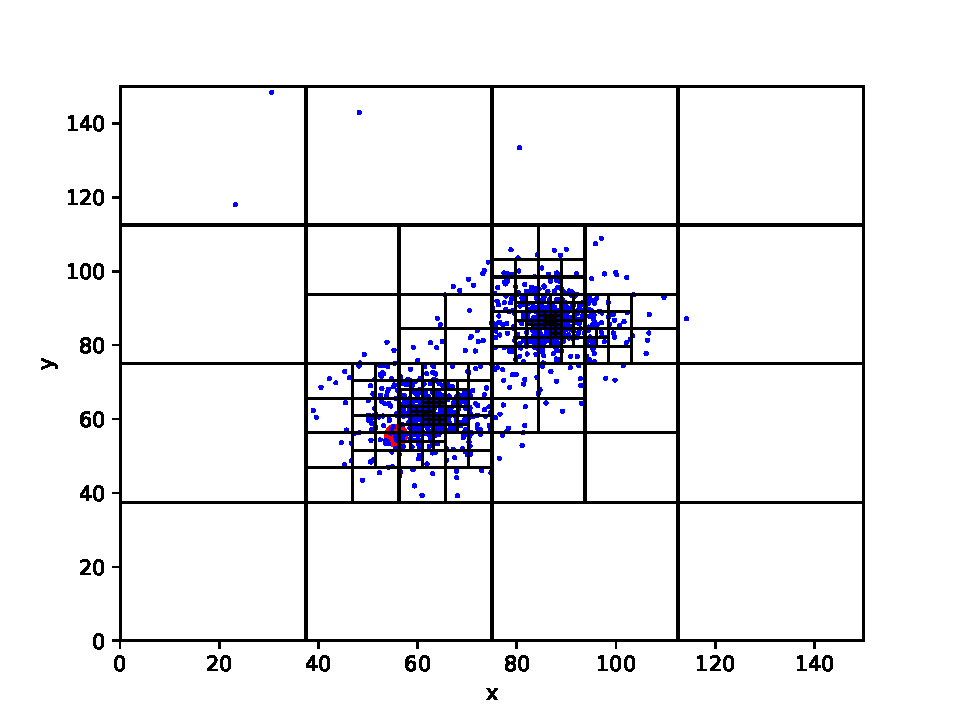
\includegraphics[width=14cm, height=8.5cm]{./Plots/7_quadtree.pdf}
\caption{A visual representation of the constructed quadtree. The blue points indicate the positions of the bodies added to the tree. The red point indicates the position of the body with index 100.}
\end{figure}
\end{quote}

\end{quote}











%\section*{\textbf{3 - Linear structure growth} \hrule} 



\subsection*{\textbf{Question 3}}
\begin{quote}

\textbf{Problem}
\begin{quote} Solve the ODE of equation \ref{eq:ode}  for the 3 given initial conditions in an matter-dominated Einstein\- de Sitter Universe. Use an appropriate numerical method. Compare the results with the analytical solution of the ODE. Plot the solution for $t = 1$ until $t = 1000$ yr, use a log\- log plot. 
\begin{equation}
\frac{d^2 D}{dt^2} + 2 \frac{\dot{a}}{a} \frac{dD}{dt} = \frac{3}{2} \omega_0 H_0^2\frac{1}{a^3}D
\label{eq:ode}
\end{equation}

\textbf{Initial conditions:}
\begin{equation*}
\text{(A)  } D(1) = 3, D'(1) = 2 \hspace*{1cm} \text{(B)  } D(1) = 10, D'(1) = - 10 \hspace*{1cm} \text{(C) } D(1) = 5, D'(1) = 0
\end{equation*}

\end{quote}

\textbf{Solution} 
\begin{quote}
The solution of this problem consist of three parts. One, a rewritten version of equation \ref{eq:ode} with the scale factor plugged in. Two, a derivation of the analytical solution. Three, a (brief) explanation on how this rewritten version is used numerically.
\\

\textbf{(1) Rewriting the ODE.}
\begin{quote}

The numerical and analytical solution both require a version of equation \ref{eq:ode} with the scale factor plugged in. For an Einstein-de Sitter Universe the scale factor and its derivative are given by, 
\begin{equation}
a(t) = \left(\frac{3}{2} H_0 t \right)^{2/3} \hspace*{1cm} \text{and} \hspace*{1cm} \dot{a}(t) = H_0 \left(\frac{3}{2} H_0 t \right)^{-1/3}
\end{equation}

Plugin this in by equation 18 and using that $\Omega_0 = 1$  results in the rewritten version,
\begin{align}
\frac{d^2D}{dt^2} + \frac{H_0 \left(\frac{3}{2} H_0 t \right)^{-1/3}}{\left(\frac{3}{2} H_0 t \right)^{2/3}} \frac{dD}{dt} - \frac{3}{2} \Omega_0 \frac{H_0^2}{\left(\frac{3}{2} H_0 t \right)^{2/3}}D &= 0 \\
\frac{d^2D}{dt^2} + \frac{4}{3t} \frac{dD}{dt} - \frac{2}{3t^2}D &= 0
\label{eq:ode2}
\end{align}
\end{quote}


\textbf{(2) Analytical solution}
\begin{quote}
The analytical solution that is required for the plots can be found by solving equation 21. The equation is solved by finding two particular solutions. These can be found by finding the values of lambda for which the the ansatz $D(t) = t^{\lambda}$ holds. Plugin in the ansatz yields,

\begin{equation}
\lambda \left(\lambda -1 \right) t^{\lambda - 2} + \frac{4}{3t} \lambda t^{\lambda -1} - \frac{2}{3t^2}t^{\lambda} = 0
\end{equation}

This simplifies to
\begin{align*}
0 & = \lambda \left( \lambda -1 \right) t^{\lambda} + \frac{4}{3} \lambda t^{\lambda} - \frac{2}{3} t^{\lambda}  \\
&= \lambda ( \lambda -1 ) + \frac{4}{3} \lambda - \frac{2}{3}  \\
&= \lambda^2 + \frac{1}{3} \lambda - \frac{2}{3} \\
&= (\lambda + 1) (\lambda - \frac{2}{3} )  \\
\end{align*}

From the above expression it can be seem that peculiar solutions of the ODE are given by,
\begin{equation}
D(t) = t^{-1} \hspace*{2cm} D(t) = t^{2/3}
\end{equation}

The general solution is the superposition of the peculiar solutions with constants and can therefore be written as,
\begin{equation}
D(t) = c_{1} t^{2/3} + c_2 t^{-1}
\end{equation}

The constants for the three initial cases can be found by calculating the derivative of the above equation and solving the system for the derivative and the non derivative.  This yields for the three cases that, 

\begin{equation}
\text{(A) } c_1 = 3, c_2 = 0 \hspace*{1cm} \text{(B) } c_1 =0, c_2 = 10 \hspace*{1cm} \text{(C) } c_1 = 3, c_2 = 2 
\end{equation}

\end{quote}


\textbf{(3) Numerical solution}
\begin{quote}
The numerical solution is obtained by first writing equation 21 as a system of first order ODE's and then by applying the Dormand\- Prince version of the Runge-kutta method. The second order ODE  can be written as a system of first order ODE's by substituting $dD/dt = u$. The system then becomes,

\begin{equation}
\large
\begin{cases} 
\frac{dD}{dt} &= u \\ 
\frac{d^2D}{d^2} &= - \frac{4}{3t}u + \frac{2}{3t^2}D 
\end{cases}
\end{equation}

The above system is as mentioned before solved with the Dormand\- Prince version of the Runge-Kutta method. The algorithm uses an adaptive step size that is initial set to $t_{step} = 0.01$ year for all cases. The code that is used to solve the ODE numerically and generates the plots is split over two files. The first file generates the plots and the second file contains the implementation of the Dormand\- Prince version of the Runge-Kutta method. The code and its output can be found below. % can be round below. The code 
\end{quote}


\newpage
 
\end{quote}

\textbf{Code - Plots}

\begin{quote}
The code that created the plots for the three given initial conditions of the ODE. % cases of the ODE. for solving the ODE for the three initial cases.generating the three plots.
\centering
\lstinputlisting{./Code/assigment_3.py}
\end{quote}

\textbf{Code - Runge-Kutta}
\begin{quote}

The code for the Dormand\- Prince version of the Runda kutta method. 

\centering
\lstinputlisting{./Code/mathlib/ode.py}
\end{quote}

\newpage

\textbf{Code - Output plot(s)}
\begin{quote}
\begin{figure}[!ht]
\centering
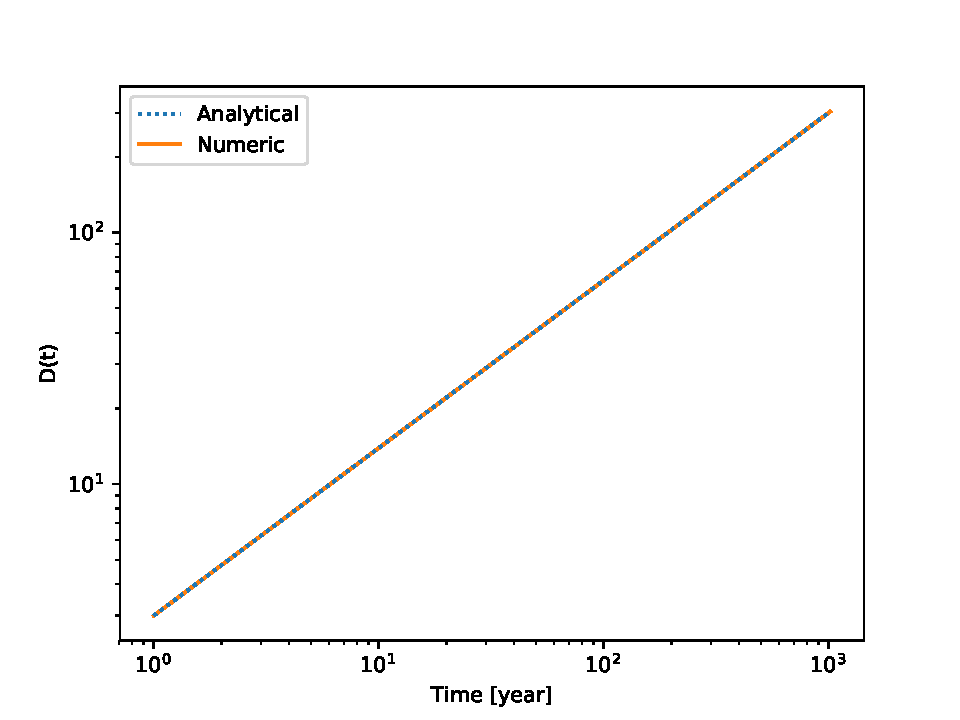
\includegraphics[width=14cm, height=8.5cm]{./Plots/3_ode_0.pdf}
\caption{The analytical (blue) and numerical (orange) solution of the ODE with initial conditions $D(1) = 3, D'(1) = -10$. The plots show that he numerical solution does not appear to have a visible deviation from the analytical solution for the given time interval.}
\end{figure}

\begin{figure}[!ht]
\centering
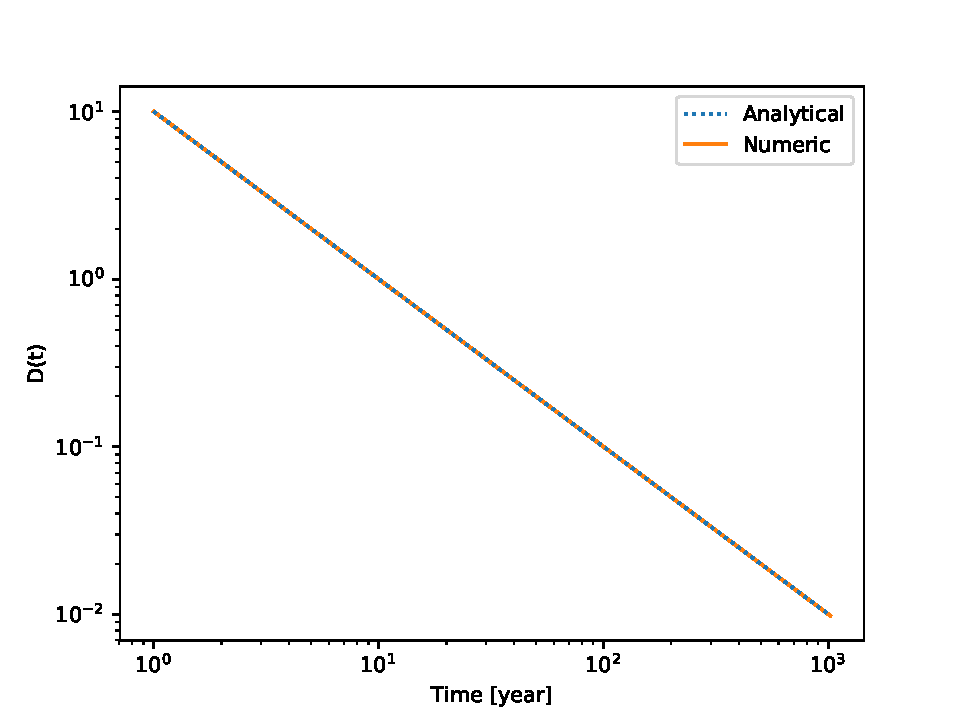
\includegraphics[width=14cm, height=8.5cm]{./Plots/3_ode_1.pdf}
\caption{The analytical (blue) and numerical solution (orange) of the ODE with initial conditions $D(1) = 10,  D'(1) = -10$. The plots show that he numerical solution does not appear to have a visible deviation from the analytical solution for the given time interval.}
\end{figure}
\newpage


\begin{figure}[!ht]
\centering
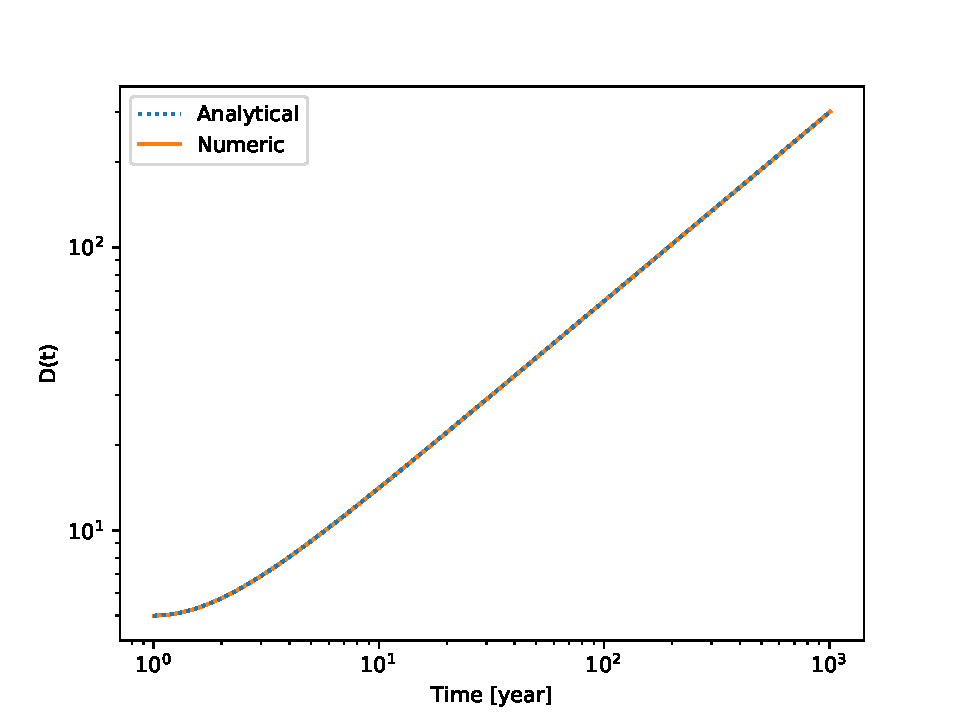
\includegraphics[width=14cm, height=8.5cm]{./Plots/3_ode_2.pdf}
\caption{The analytical (blue) and numerical (orange) solution of the ODE with initial conditions $D(1) = 5,  D'(1) = 0$. The plots show that he numerical solution does not appear to have a visible deviation from the analytical solution for the given time interval.}
\end{figure}

\end{quote}
\end{quote}












  







\end{document}
